\documentclass[11pt,a4paper]{article}
\usepackage[utf8]{inputenc}
\IfFileExists{lmodern.sty}{\usepackage[T1]{fontenc}\usepackage{lmodern}}{}
\usepackage{mathrsfs}
\usepackage[english]{babel}
\usepackage[a4paper,margin=25mm]{geometry}
\usepackage[expansion=false]{microtype}
\usepackage{amsmath,amssymb}
\usepackage{placeins}
\AtBeginDocument{\RenewCommandCopy\qty\SI}
\usepackage{tikz}
\usepackage{stmaryrd}
\usepackage{esint}
\usepackage{graphicx}
\usetikzlibrary{arrows.meta}
\usepackage[hidelinks]{hyperref}
\usepackage{enumitem}
\definecolor{OptBlue}{HTML}{205681}
\definecolor{OptBackground}{HTML}{F3F7FB}
\definecolor{OptGrey}{HTML}{586779}
\usepackage{nicefrac}
\usepackage[most]{tcolorbox}
\usepackage{physics}
\usepackage{mathdots}
\usepackage{yhmath}
\usepackage{cancel}
\usepackage{color}
\usepackage{siunitx}
\usepackage{array}
\usepackage{multirow}
\usepackage{gensymb}
\usepackage{tabularx}
\usepackage{extarrows}
\usepackage{booktabs}
\usetikzlibrary{fadings}
\usetikzlibrary{patterns}
\usetikzlibrary{shadows.blur}
\usetikzlibrary{shapes}

\definecolor{accent}{HTML}{1F3A5F}

\newtcolorbox{fundamentalproblem}{
    enhanced,
    breakable,
    colback=OptBackground,
    colframe=OptBackground,
    boxrule=0pt,
    borderline west={2.8pt}{0pt}{OptBlue},
    arc=1mm,
    left=5mm,
    right=5mm,
    top=4mm,
    bottom=4mm,
    before skip=12pt,
    after skip=12pt
}

\newcommand{\methodquestion}[2]{%
    \par\addvspace{0.8em}%
    \noindent\textit{#1}\par
    \vspace{0.25em}%
    \noindent\hspace*{0.4em}%
    {\color{black!40}\vrule width 1.2pt}%
    \hspace{0.8em}%
    \begin{minipage}[t]{\dimexpr\linewidth-1.5em\relax}
        #2
    \end{minipage}%
    \par
}

\definecolor{flowblue}{HTML}{17546D}
\definecolor{shockred}{HTML}{9A3D32}
\renewcommand{\dd}{\mathrm d}
\renewcommand{\tr}{\operatorname{tr}}
\newcommand{\naca}{NACA~0012}
\newcommand{\dpartial}[1]{\partial_{\boxslash}^{2}#1}

\title{Mesh Adaptation}
\author{}
\date{}

\begin{document}
\maketitle


\section{Problem statement}

\begin{minipage}[c]{0.65\textwidth}
    \raggedright
    We consider a two-dimensional fluid domain
    $\Omega$, discretized using an anisotropic
    triangular mesh.  Let $\mathcal{T}$ denote the set of all triangles in the mesh, and let $\mathcal{V}(T)$ denote
    the set of vertices of a triangle $T$. Thus,
    \(
        \mathcal{V}(T)
        = \left\{
            \mathbf{x}_1,
            \mathbf{x}_2,
            \mathbf{x}_3
          \right\},
    \)
    where
    \(
        \mathbf{x}_i = \left(x_i ,y_i\right)
        \in \mathbb{R}^2.
    \)

\end{minipage}
\hfill
\begin{minipage}[c]{0.32\textwidth}
    \centering

     \resizebox{\linewidth}{!}{%
        

\tikzset{every picture/.style={line width=0.5pt}} %set default line width to 0.75pt        

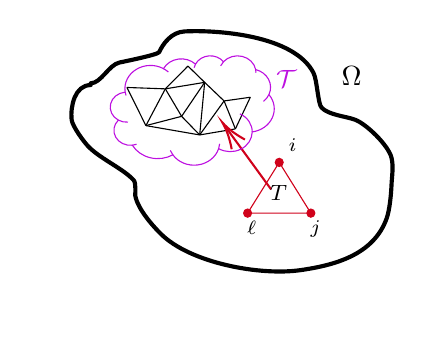
\begin{tikzpicture}[
    x=0.9pt,
    y=0.9pt,
    yscale=-1,
    xscale=1,
    % scale=0.65,
    % % transform shape
]
\path (0,128); %set diagram left start at 0, and has height of 128

%Shape: Free Drawing [id:dp28662961249906116] 
\draw  [line width=1.5] [line join = round][line cap = round] (25.31,35.64) .. controls (18.94,35.64) and (17.1,44.17) .. (17.64,49.53) .. controls (17.92,52.21) and (22.84,58.86) .. (24.67,60.64) .. controls (29.81,65.6) and (38.32,69.21) .. (42.56,73.83) .. controls (43.61,74.97) and (43.12,79.63) .. (43.2,80.08) .. controls (44.21,85.57) and (50.5,92.45) .. (53.42,95.35) .. controls (65.34,107.18) and (93.49,112.3) .. (109.65,109.94) .. controls (122.74,108.02) and (138.85,104.08) .. (144.15,89.11) .. controls (145.32,85.8) and (145.91,79.63) .. (146.07,75.91) .. controls (146.22,72.21) and (146.96,68.38) .. (146.07,64.8) .. controls (144.81,59.74) and (135.79,51.13) .. (131.37,49.53) .. controls (127.62,48.17) and (120.68,47.63) .. (117.96,44.66) .. controls (116.54,43.13) and (116.21,33.6) .. (114.76,30.78) .. controls (106.98,15.55) and (75.94,13.44) .. (63.01,14.11) .. controls (57.69,14.39) and (54.36,19.01) .. (52.78,22.44) .. controls (52.32,23.45) and (38.34,26.28) .. (36.81,26.61) .. controls (32.63,27.52) and (29.4,34.94) .. (25.31,34.94) ;
%Straight Lines [id:da21743711677891986] 
\draw    (39.85,36.61) -- (47.47,51.93) ;
%Straight Lines [id:da21156975196861816] 
\draw    (47.47,51.93) -- (55.27,37.17) ;
%Straight Lines [id:da071960796489286] 
\draw    (55.27,37.17) -- (39.85,36.61) ;
%Straight Lines [id:da4873435641892746] 
\draw    (64.35,28.02) -- (55.27,37.17) ;
%Straight Lines [id:da34293143567655815] 
\draw    (55.27,37.17) -- (71.06,34.56) ;
%Straight Lines [id:da053908988647655476] 
\draw    (64.35,28.02) -- (71.06,34.56) ;
%Straight Lines [id:da035764812836924675] 
\draw    (71.06,34.56) -- (61.81,48.2) ;
%Straight Lines [id:da11995141775636042] 
\draw    (61.81,48.2) -- (55.27,37.17) ;
%Straight Lines [id:da5090490449231705] 
\draw    (61.81,48.2) -- (47.47,51.93) ;
%Straight Lines [id:da49066648790192713] 
\draw    (69.06,55.67) -- (47.47,51.93) ;
%Straight Lines [id:da2538401588440199] 
\draw    (69.06,55.67) -- (61.81,48.2) ;
%Straight Lines [id:da8251904081975683] 
\draw    (71.06,34.56) -- (69.06,55.67) ;
%Straight Lines [id:da7581764144619609] 
\draw    (71.06,34.56) -- (78.86,42.03) ;
%Straight Lines [id:da7927189639662129] 
\draw    (69.06,55.67) -- (83.4,53.24) ;
%Straight Lines [id:da8413968971679558] 
\draw    (78.86,42.03) -- (69.06,55.67) ;
%Straight Lines [id:da38935640303030195] 
\draw    (78.86,42.03) -- (83.4,53.24) ;
%Straight Lines [id:da0249824130205758] 
\draw    (89.39,40.54) -- (83.4,53.24) ;
%Straight Lines [id:da8027838216009948] 
\draw    (89.39,40.54) -- (78.86,42.03) ;
%Shape: Triangle [id:dp47295493723046833] 
\draw  [color={rgb, 255:red, 208; green, 2; blue, 27 }  ,draw opacity=1 ] (101,66.7) -- (113.7,87.06) -- (88.3,87.06) -- cycle ;
%Shape: Ellipse [id:dp36287656076302666] 
\draw  [color={rgb, 255:red, 208; green, 2; blue, 27 }  ,draw opacity=1 ][fill={rgb, 255:red, 208; green, 2; blue, 27 }  ,fill opacity=1 ] (99.41,66.7) .. controls (99.41,65.79) and (100.12,65.06) .. (101,65.06) .. controls (101.88,65.06) and (102.59,65.79) .. (102.59,66.7) .. controls (102.59,67.6) and (101.88,68.33) .. (101,68.33) .. controls (100.12,68.33) and (99.41,67.6) .. (99.41,66.7) -- cycle ;
%Shape: Ellipse [id:dp7741968050608962] 
\draw  [color={rgb, 255:red, 208; green, 2; blue, 27 }  ,draw opacity=1 ][fill={rgb, 255:red, 208; green, 2; blue, 27 }  ,fill opacity=1 ] (112.11,87.06) .. controls (112.11,86.16) and (112.82,85.43) .. (113.7,85.43) .. controls (114.58,85.43) and (115.29,86.16) .. (115.29,87.06) .. controls (115.29,87.97) and (114.58,88.7) .. (113.7,88.7) .. controls (112.82,88.7) and (112.11,87.97) .. (112.11,87.06) -- cycle ;
%Shape: Ellipse [id:dp0857892517199157] 
\draw  [color={rgb, 255:red, 208; green, 2; blue, 27 }  ,draw opacity=1 ][fill={rgb, 255:red, 208; green, 2; blue, 27 }  ,fill opacity=1 ] (86.71,87.06) .. controls (86.71,86.16) and (87.42,85.43) .. (88.3,85.43) .. controls (89.17,85.43) and (89.89,86.16) .. (89.89,87.06) .. controls (89.89,87.97) and (89.17,88.7) .. (88.3,88.7) .. controls (87.42,88.7) and (86.71,87.97) .. (86.71,87.06) -- cycle ;
%Straight Lines [id:da5398430161100607] 
\draw [color={rgb, 255:red, 208; green, 2; blue, 27 }  ,draw opacity=1 ][line width=0.75]    (97.73,77.53) -- (79.31,52.24) ;
\draw [shift={(78.14,50.63)}, rotate = 53.93] [color={rgb, 255:red, 208; green, 2; blue, 27 }  ,draw opacity=1 ][line width=0.75]    (10.93,-3.29) .. controls (6.95,-1.4) and (3.31,-0.3) .. (0,0) .. controls (3.31,0.3) and (6.95,1.4) .. (10.93,3.29)   ;
%Shape: Cloud [id:dp2091191547824247] 
\draw  [color={rgb, 255:red, 189; green, 16; blue, 224 }  ,draw opacity=1 ] (39.13,38.36) .. controls (38.6,34.82) and (40.34,31.32) .. (43.62,29.34) .. controls (46.89,27.35) and (51.12,27.24) .. (54.52,29.05) .. controls (55.72,26.99) and (57.92,25.57) .. (60.46,25.21) .. controls (62.99,24.86) and (65.56,25.61) .. (67.39,27.25) .. controls (68.41,25.38) and (70.42,24.13) .. (72.71,23.93) .. controls (74.99,23.74) and (77.23,24.63) .. (78.62,26.28) .. controls (80.47,24.31) and (83.41,23.47) .. (86.18,24.14) .. controls (88.94,24.82) and (91.03,26.88) .. (91.54,29.43) .. controls (93.81,29.99) and (95.7,31.42) .. (96.72,33.34) .. controls (97.74,35.27) and (97.79,37.51) .. (96.87,39.47) .. controls (99.1,42.11) and (99.62,45.63) .. (98.24,48.71) .. controls (96.86,51.79) and (93.78,53.98) .. (90.15,54.45) .. controls (90.12,57.34) and (88.37,60) .. (85.58,61.39) .. controls (82.79,62.78) and (79.38,62.7) .. (76.67,61.17) .. controls (75.52,64.63) and (72.28,67.18) .. (68.35,67.71) .. controls (64.41,68.25) and (60.5,66.67) .. (58.29,63.66) .. controls (55.58,65.14) and (52.33,65.57) .. (49.27,64.84) .. controls (46.21,64.12) and (43.6,62.3) .. (42.03,59.8) .. controls (39.26,60.1) and (36.59,58.79) .. (35.33,56.54) .. controls (34.08,54.29) and (34.51,51.56) .. (36.41,49.72) .. controls (33.94,48.4) and (32.68,45.78) .. (33.29,43.23) .. controls (33.89,40.68) and (36.23,38.77) .. (39.08,38.5) ; \draw  [color={rgb, 255:red, 189; green, 16; blue, 224 }  ,draw opacity=1 ] (36.41,49.72) .. controls (37.58,50.34) and (38.92,50.63) .. (40.27,50.53)(42.03,59.8) .. controls (42.61,59.74) and (43.18,59.61) .. (43.72,59.41)(58.29,63.66) .. controls (57.88,63.1) and (57.54,62.51) .. (57.27,61.89)(76.67,61.17) .. controls (76.88,60.53) and (77.02,59.88) .. (77.08,59.23)(90.15,54.45) .. controls (90.17,51.37) and (88.25,48.55) .. (85.2,47.2)(96.87,39.47) .. controls (96.37,40.52) and (95.62,41.45) .. (94.66,42.19)(91.54,29.43) .. controls (91.62,29.85) and (91.66,30.28) .. (91.65,30.71)(78.62,26.28) .. controls (78.16,26.78) and (77.78,27.33) .. (77.49,27.92)(67.39,27.25) .. controls (67.14,27.7) and (66.96,28.17) .. (66.84,28.66)(54.52,29.05) .. controls (55.24,29.43) and (55.9,29.89) .. (56.5,30.42)(39.13,38.36) .. controls (39.2,38.85) and (39.32,39.33) .. (39.48,39.8) ;

% Text Node
\draw (103.7,56.27) node [anchor=north west][inner sep=0.75pt]  [font=\scriptsize]  {$i$};
% Text Node
\draw (112.46,89.15) node [anchor=north west][inner sep=0.75pt]  [font=\scriptsize]  {$j$};
% Text Node
\draw (87.06,89.15) node [anchor=north west][inner sep=0.75pt]  [font=\scriptsize]  {$\ell $};
% Text Node
\draw (96.32,74.89) node [anchor=north west][inner sep=0.75pt]  [font=\footnotesize]  {$T$};
% Text Node
\draw (98.67,28.73) node [anchor=north west][inner sep=0.75pt]  [font=\small,color={rgb, 255:red, 189; green, 16; blue, 224 }  ,opacity=1 ]  {$\mathcal{T}$};
% Text Node
\draw (125,27.15) node [anchor=north west][inner sep=0.75pt]  [font=\normalsize]  {$\Omega $};


\end{tikzpicture}%
    }

\end{minipage}


\noindent
The mesh refinement is based on the study of the density $\rho$ since it's the relevant parameter for our project where the critical phenomenon are mainly shocks. Thus, we consider that we know at any vertex the numerical density $\rho_i$. \\

\noindent
Over a triangle $T$, the local density $\rho_h$ is fitted over a plan by an \emph{piecewise affine} interpolation through the three nodal values on each triangle, also called a $P_1$ interpolation. We write then :
\begin{equation}
    \rho_h(x,y)\big|_T = a_T + b_T x + c_T y .
\end{equation}

\noindent
The values at the three vertices determine the coefficients \(a_T,b_T,c_T\). \\

\noindent
In a region where $\rho$ behaves spatially slowly, a large $T$ could be sufficient. However, in the vicinity of a shock, the numerical density is ideally discontinuous, which is represented by a sudden change of value. There, we must get the vertices closer in the normal direction of the shock. In the tangential direction, we have a low evolution of the density, so we can keep a greater distance between the vertices. Hence, this introduces an anisotropic adaptation of the triangles, based on refining the grid locally depending on the directions of the critical phenomenons.\\

\noindent
To do so, three fundamental questions must be addressed:
\begin{table}[htbp]
\centering
\renewcommand{\arraystretch}{1.15}
\begin{tabularx}{\linewidth}{
    >{\raggedright\arraybackslash}X
    >{\raggedright\arraybackslash}X
}
\toprule
\textbf{Question} & \textbf{Underlying principle} \\
\midrule
Where is affine interpolation less accurate?
& Local curvature of the field. \\

Along which directions should the mesh be refined?
& Principal directions of curvature. \\

How should the available nodes be distributed?
& Global node budget and local error model. \\
\bottomrule
\end{tabularx}
\end{table}

\noindent
The first 2 points are actually handled through the use of the Hessian. The metric of the grid translate the Hessian information into a physical size and solve the global budget.



\section{How the Hessian is used to refine ?}
\subsection{Interpolation error between two vertices}

% Consider a triangle $T$. We take one of its edge of length \(h\). Let \(s\) be the local coordinate oriented by $\mathbf{e}$ unitarian along the edge from its first vertex and \(r(s)\) the density along that line defined by : $r(s)=\rho(\mathbf{x_0}+s\mathbf{e})$ where $s\in[0,h]$. 

% Given the two endpoint values \(r(0)\) and \(r(h)\), the linear
% interpolant \(I_h r\) joins them with a straight line. At the midpoint,
% it gives the average of the endpoint values.
% \[
%   (I_h r)(h/2)=\frac{r(0)+r(h)}{2}.
% \]

\noindent
\begin{minipage}[c]{0.35\linewidth}
\vspace{-1 cm}
    \centering
    \resizebox{0.8\linewidth}{!}{%
        

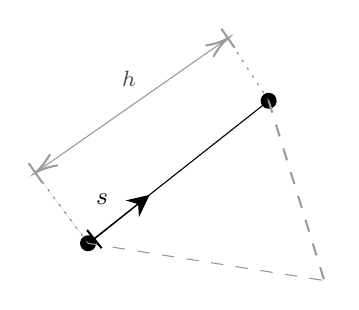
\begin{tikzpicture}[x=0.75pt,y=0.75pt,yscale=-1,xscale=1]
%uncomment if require: \path (0,300); %set diagram left start at 0, and has height of 300

%Straight Lines [id:da5193201442794912] 
\draw    (100,122) -- (187,53.33) ;
\draw [shift={(187,53.33)}, rotate = 321.72] [color={rgb, 255:red, 0; green, 0; blue, 0 }  ][fill={rgb, 255:red, 0; green, 0; blue, 0 }  ][line width=0.75]      (0, 0) circle [x radius= 3.35, y radius= 3.35]   ;
\draw [shift={(100,122)}, rotate = 321.72] [color={rgb, 255:red, 0; green, 0; blue, 0 }  ][fill={rgb, 255:red, 0; green, 0; blue, 0 }  ][line width=0.75]      (0, 0) circle [x radius= 3.35, y radius= 3.35]   ;
%Straight Lines [id:da7789605754173338] 
\draw [color={rgb, 255:red, 155; green, 155; blue, 155 }  ,draw opacity=1 ] [dash pattern={on 4.5pt off 4.5pt}]  (100,122) -- (216.6,140.4) ;
%Straight Lines [id:da16183660515131726] 
\draw [color={rgb, 255:red, 155; green, 155; blue, 155 }  ,draw opacity=1 ][line width=0.75]  [dash pattern={on 4.5pt off 4.5pt}]  (187,53.33) -- (213.8,140) ;
%Straight Lines [id:da8821511551285445] 
\draw    (103,120) -- (127.32,100.54) ;
\draw [shift={(129.67,98.67)}, rotate = 141.34] [fill={rgb, 255:red, 0; green, 0; blue, 0 }  ][line width=0.08]  [draw opacity=0] (10.72,-5.15) -- (0,0) -- (10.72,5.15) -- (7.12,0) -- cycle    ;
\draw [shift={(103,120)}, rotate = 141.34] [color={rgb, 255:red, 0; green, 0; blue, 0 }  ][line width=0.75]    (0,5.59) -- (0,-5.59)   ;
%Straight Lines [id:da04682054555931536] 
\draw [color={rgb, 255:red, 128; green, 128; blue, 128 }  ,draw opacity=1 ][fill={rgb, 255:red, 74; green, 144; blue, 226 }  ,fill opacity=1 ] [dash pattern={on 0.84pt off 2.51pt}]  (100,122) -- (74.6,88) ;
%Straight Lines [id:da26884514590564546] 
\draw [color={rgb, 255:red, 128; green, 128; blue, 128 }  ,draw opacity=1 ] [dash pattern={on 0.84pt off 2.51pt}]  (187,53.33) -- (167.4,23.2) ;
%Straight Lines [id:da1403183000892151] 
\draw [color={rgb, 255:red, 155; green, 155; blue, 155 }  ,draw opacity=1 ]   (74.6,88) -- (167.4,23.2) ;
\draw [shift={(167.4,23.2)}, rotate = 145.07] [color={rgb, 255:red, 155; green, 155; blue, 155 }  ,draw opacity=1 ][line width=0.75]    (0,5.59) -- (0,-5.59)(10.93,-3.29) .. controls (6.95,-1.4) and (3.31,-0.3) .. (0,0) .. controls (3.31,0.3) and (6.95,1.4) .. (10.93,3.29)   ;
\draw [shift={(74.6,88)}, rotate = 325.07] [color={rgb, 255:red, 155; green, 155; blue, 155 }  ,draw opacity=1 ][line width=0.75]    (0,5.59) -- (0,-5.59)(10.93,-3.29) .. controls (6.95,-1.4) and (3.31,-0.3) .. (0,0) .. controls (3.31,0.3) and (6.95,1.4) .. (10.93,3.29)   ;

% Text Node
\draw (102.67,96.73) node [anchor=north west][inner sep=0.75pt]  [font=\small]  {$s$};
% Text Node
\draw (115.2,37.8) node [anchor=north west][inner sep=0.75pt]  [font=\footnotesize,color={rgb, 255:red, 74; green, 74; blue, 74 }  ,opacity=1 ]  {$h$};


\end{tikzpicture}
%
    }
\end{minipage}%
\hfill
\begin{minipage}[c]{0.62\linewidth}

    Consider a triangle $T$ and one of its edges
    of length $h$.
    Let $s\in[0,h]$ be the local coordinate
    along the edge, measured from its first
    vertex $\mathbf{x}_0$, and let $\mathbf{e}$
    be the corresponding unit tangent vector.
    The density restricted to this edge is
    defined as
    \(
        r(s)=\rho(\mathbf{x}_0+s\mathbf{e}).
    \)
    Given the endpoint values $r(0)$ and
    $r(h)$, the linear interpolant $I_h r$
    connects them by a straight line.
    At the midpoint, its value is
    \begin{equation}
        \boxed{
        \left(I_h r\right)\left(\frac{h}{2}\right)
        =\frac{r(0)+r(h)}{2}
        }
    \end{equation}
    \vspace{6pt}

\end{minipage}


% If \(\rho\) increases at a constant rate along the edge, the
% interpolant gives the exact midpoint value even for a steep slope.
% When the slope varies, the straight line deviates from the density
% curve. 

\noindent
\begin{minipage}[c]{0.8\linewidth}
    \raggedright
    If $\rho$ increases at a constant rate along the edge,
    the interpolant gives the exact midpoint value, even
    for a steep slope. When the slope varies, the straight line deviates from the density curve.
\end{minipage}%
\hfill
\begin{minipage}[c]{0.2\linewidth}
    \centering
    \resizebox{\linewidth}{!}{%
        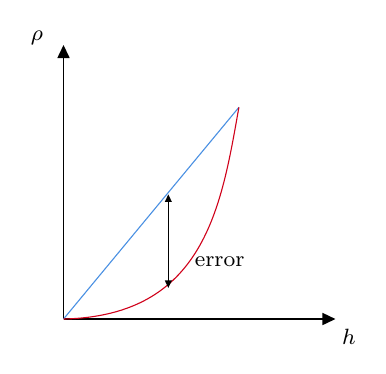
\begin{tikzpicture}[x=0.75pt,y=0.75pt,yscale=-1,xscale=1]
        %uncomment if require: \path (0,323); %set diagram left start at 0, and has height of 323
        
        %Straight Lines [id:da08138028104019213] 
        \draw    (89.5,220.5) -- (89.5,91.5) ;
        \draw [shift={(89.5,88.5)}, rotate = 90] [fill={rgb, 255:red, 0; green, 0; blue, 0 }  ][line width=0.08]  [draw opacity=0] (6.25,-3) -- (0,0) -- (6.25,3) -- cycle    ;
        %Straight Lines [id:da57229455725135] 
        \draw    (89.5,220.5) -- (217.5,220.5) ;
        \draw [shift={(220.5,220.5)}, rotate = 180] [fill={rgb, 255:red, 0; green, 0; blue, 0 }  ][line width=0.08]  [draw opacity=0] (6.25,-3) -- (0,0) -- (6.25,3) -- cycle    ;
        %Straight Lines [id:da22518428796341516] 
        \draw [color={rgb, 255:red, 74; green, 144; blue, 226 }  ,draw opacity=1 ]   (89.5,220.5) -- (174,118.5) ;
        %Curve Lines [id:da012038799493175434] 
        \draw [color={rgb, 255:red, 208; green, 2; blue, 27 }  ,draw opacity=1 ]   (89.5,220.5) .. controls (157.5,219) and (165.5,166.5) .. (174,118.5) ;
        %Straight Lines [id:da6432642344844286] 
        \draw    (140,163.5) -- (140,202.5) ;
        \draw [shift={(140,205.5)}, rotate = 270] [fill={rgb, 255:red, 0; green, 0; blue, 0 }  ][line width=0.08]  [draw opacity=0] (3.57,-1.72) -- (0,0) -- (3.57,1.72) -- cycle    ;
        \draw [shift={(140,160.5)}, rotate = 90] [fill={rgb, 255:red, 0; green, 0; blue, 0 }  ][line width=0.08]  [draw opacity=0] (3.57,-1.72) -- (0,0) -- (3.57,1.72) -- cycle    ;
        
        % Text Node
        \draw (72.5,80.4) node [anchor=north west][inner sep=0.75pt]  [font=\footnotesize]  {$\rho$};
        % Text Node
        \draw (222.5,223.9) node [anchor=north west][inner sep=0.75pt]  [font=\footnotesize]  {$h$};
        % Text Node
        \draw (151.5,189.4) node [anchor=north west][inner sep=0.75pt]  [font=\footnotesize]  {$\text{error}$};
        
        \end{tikzpicture}%
    }
\end{minipage}

\vspace{3pt}
\noindent
Let's quantify this error through a Taylor expansion. Let $r\in \mathcal{C}^2([0,h])$. We expand around $h/2$. Then the Taylor-Lagrange expansion reads : 
\begin{align}
    \exists \,\xi^- \in \left]0,\tfrac{h}{2}\right[ :\qquad & r(0) = r\left(\tfrac{h}{2}\right) -\tfrac{h}{2}r'\left(\tfrac{h}{2}\right) + \tfrac{h^2}{8} r''\left(\xi^-\right) \\
    \exists \,\xi^+ \in \left]\tfrac{h}{2},h\right[ : \qquad & r(0) = r\left(\tfrac{h}{2}\right) +\tfrac{h}{2}r'\left(\tfrac{h}{2}\right) + \tfrac{h^2}{8} r''\left(\xi^+\right)
\end{align}
\noindent
So we have :
\begin{align}
    \left(I_hr\right)\left(\tfrac{h}{2}\right)  =\frac{r(0)+r(h)} {2} = r\left(\tfrac{h}{2}\right) + \frac{h^2}{8} \frac{r''\left(\xi^+\right)+r''\left(\xi^-\right)}{2}
\end{align}

\noindent
Since \(r\) is $\mathcal{C}^2$ on the segment, somewhere between $\xi^+$ and $\xi^-$, the mean of the density is reached, we can say that : $\exists \,\xi \in \left]0,h\right[$ where $r''(\xi)=\tfrac{r''\left(\xi^+\right)+r''\left(\xi^-\right)}{2}$. Then, the error is given by : 
\begin{equation}
  \boxed{  
  \left(I_hr\right)\left(\tfrac{h}{2}\right)  - r\left(\tfrac{h}{2}\right)=\tfrac{h^2}{8}\,r''(\xi),
  \qquad 0<\xi<h }
\end{equation}
The factor \(\lvert r''\rvert\) scales the rate of change of the
slope, and the factor \(h^2\) accounts for the edge size. At comparable
curvature, dividing the edge length by 2 reduces the error scale by a factor of 4.



\subsection{Directional curvature in 2D}

\noindent
The curvature along an edge depends on its orientation. The second
derivatives of \(\rho\) are retrieved from the
\emph{Hessian}.
\begin{equation}
  \mathbf{H}_\rho=\nabla^2\rho =
  \begin{bmatrix}
    \partial_{xx}\rho & \partial_{xy}\rho\\
    \partial_{yx}\rho & \partial_{yy}\rho
  \end{bmatrix}
\end{equation}

\noindent
Along a straight line \(\mathbf x(s)=\mathbf x_0+s\mathbf e\), the chain rule gives
\begin{equation}
  r''(s)=\mathbf e^\top \mathbf{H}_\rho(\mathbf x(s))\,\mathbf e .
\end{equation}

\noindent
We enforce the Hessian to be symmetrical since the field is mainly smooth and regular. Indeed, for a smooth field, the mixed partial derivatives coincide. To enforce the symmetry, we apply the average of the off-diagonal terms : 

\begin{equation}
    \dpartial{\rho} = \frac{\partial_{xy}\rho + \partial_{yx}\rho}{2} \quad \Rightarrow \quad \widehat{\mathbf{H}}_{\rho} =\begin{bmatrix}
\partial_{xx}\rho & \dpartial{\rho} \\
 \dpartial{\rho} & \partial_{yy}\rho 
\end{bmatrix}
\end{equation}

\noindent
Now the Hessian is symmetrical, and diagonazible. It therefore has two orthogonal eigenvector directions \(\mathbf e_\mathrm{I},\mathbf e_\mathrm{II}\). The second directional derivative
along \(\mathbf e_a\) equals the corresponding eigenvalue \(\lambda_a\),
for \(a=\mathrm{I},\mathrm{II}\). The magnitude of the interpolation error depends on
\(\lvert\lambda_a\rvert\), whether the slope of \(\rho\) increases or
decreases in that direction.\\

\noindent
\begin{minipage}[c]{0.30\linewidth}
\vspace{-1 cm}
    \centering
    \resizebox{0.95\linewidth}{!}{%
        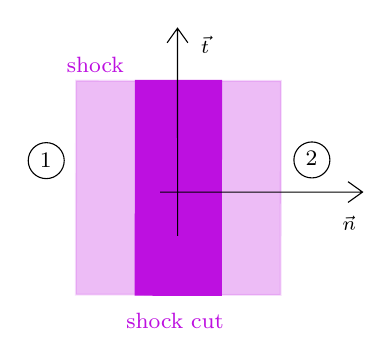
\begin{tikzpicture}[x=0.75pt,y=0.75pt,yscale=-1,xscale=1]
        %uncomment if require: \path (0,549); %set diagram left start at 0, and has height of 549
        
        %Shape: Rectangle [id:dp12460027122976491] 
        \draw  [color={rgb, 255:red, 189; green, 16; blue, 224 }  ,draw opacity=1 ][fill={rgb, 255:red, 189; green, 16; blue, 224 }  ,fill opacity=1 ][line width=0.75]  (246.23,66.54) -- (287.23,66.59) -- (287.11,169.64) -- (246.1,169.59) -- cycle ;
        %Shape: Rectangle [id:dp27812198356410855] 
        \draw  [color={rgb, 255:red, 189; green, 16; blue, 224 }  ,draw opacity=0.13 ][fill={rgb, 255:red, 189; green, 16; blue, 224 }  ,fill opacity=0.28 ][line width=0.75]  (217.4,66.5) -- (316.06,66.63) -- (315.94,169.68) -- (217.27,169.56) -- cycle ;
        %Shape: Axis 2D [id:dp38754383778692114] 
        \draw [color={rgb, 255:red, 0; green, 0; blue, 0 }  ,draw opacity=1 ] (257.85,120.19) -- (355.4,120.14)(266.24,41.21) -- (266.3,141.21) (348.4,115.14) -- (355.4,120.14) -- (348.41,125.14) (261.25,48.22) -- (266.24,41.21) -- (271.25,48.21)  ;
        %Shape: Circle [id:dp470407620687861] 
        \draw   (194.33,105) .. controls (194.33,100.21) and (198.21,96.33) .. (203,96.33) .. controls (207.79,96.33) and (211.67,100.21) .. (211.67,105) .. controls (211.67,109.79) and (207.79,113.67) .. (203,113.67) .. controls (198.21,113.67) and (194.33,109.79) .. (194.33,105) -- cycle ;
        %Shape: Circle [id:dp4934976878072427] 
        \draw   (322.33,104.67) .. controls (322.33,99.88) and (326.21,96) .. (331,96) .. controls (335.79,96) and (339.67,99.88) .. (339.67,104.67) .. controls (339.67,109.45) and (335.79,113.33) .. (331,113.33) .. controls (326.21,113.33) and (322.33,109.45) .. (322.33,104.67) -- cycle ;
        
        % Text Node
        \draw (344.19,130.89) node [anchor=north west][inner sep=0.75pt]  [font=\scriptsize,rotate=-357.57]  {$\vec{n}$};
        % Text Node
        \draw (276.09,43.91) node [anchor=north west][inner sep=0.75pt]  [font=\scriptsize,rotate=-358.08]  {$\vec{t}$};
        % Text Node
        \draw (211.67,54) node [anchor=north west][inner sep=0.75pt]  [font=\footnotesize] [align=left] {\textcolor[rgb]{0.74,0.06,0.88}{shock}};
        % Text Node
        \draw (240.33,177.33) node [anchor=north west][inner sep=0.75pt]  [font=\footnotesize] [align=left] {\textcolor[rgb]{0.74,0.06,0.88}{shock cut}};
        % Text Node
        \draw (198.67,100.33) node [anchor=north west][inner sep=0.75pt]  [font=\footnotesize] [align=left] {1};
        % Text Node
        \draw (326.67,99.33) node [anchor=north west][inner sep=0.75pt]  [font=\footnotesize] [align=left] {2\\};
        
        \end{tikzpicture}%
    }
\end{minipage}%
\hfill
\begin{minipage}[c]{0.68\linewidth}
    \raggedright

    Near a locally straight portion of the shock, let
    $\mathbf n$ and $\mathbf t$ denote the unit normal
    and tangent vectors, respectively. Since the density
    varies primarily with the normal distance $s$, we may
    write locally
    \[
        \rho(\mathbf x)\simeq R(s),
    \]
    where $R$ denotes the density profile along the
    shock cut. It follows that
    \begin{equation}
        H_\rho \simeq R''(s)\,\mathbf n\mathbf n^\top,
        \qquad
        \mathbf n^\top H_\rho \mathbf n \simeq R''(s),
        \qquad
        \mathbf t^\top H_\rho \mathbf t \simeq 0.
    \end{equation}
\vspace{3pt}
\end{minipage}

\noindent
\begin{minipage}[c]{0.63\linewidth}
    \raggedright

    A normal edge and a tangential edge of equal length can
    therefore exhibit very different interpolation errors.
    The dominant curvature may also change sign across the
    shock band. For an S-shaped transition, for example,
    $R''$ vanishes at the inflection point and has opposite
    signs on either side.

    Our indicator measures the curvature of the numerical
    transition on the current mesh. The $h^2$ interpolation
    formula applies to smooth portions of the profile, since
    an ideal shock is a discontinuity in $\rho$.

\end{minipage}%
\hfill
\begin{minipage}[c]{0.35\linewidth}
    \centering
    \resizebox{0.95\linewidth}{!}{%
        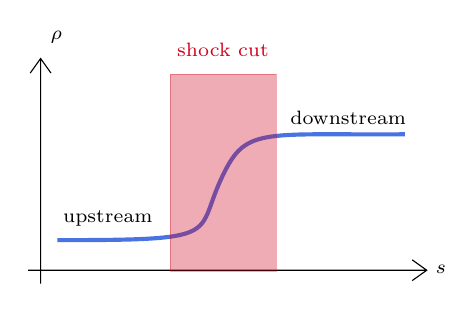
\begin{tikzpicture}[x=0.75pt,y=0.75pt,yscale=-1,xscale=1]
        %uncomment if require: \path (0,300); %set diagram left start at 0, and has height of 300
        
        %Shape: Axis 2D [id:dp9844158106254359] 
        \draw  (88,165) -- (280,165)(93.96,63) -- (93.96,171.5) (273,160) -- (280,165) -- (273,170) (88.96,70) -- (93.96,63) -- (98.96,70)  ;
        %Curve Lines [id:da06205479091784327] 
        \draw [color={rgb, 255:red, 74; green, 115; blue, 226 }  ,draw opacity=1 ][line width=1.5]    (102,150.5) .. controls (182,150.5) and (168.5,148.5) .. (180.5,122) .. controls (192.5,95.5) and (198,100) .. (269.5,99.5) ;
        %Shape: Rectangle [id:dp3735781289450384] 
        \draw  [color={rgb, 255:red, 208; green, 2; blue, 27 }  ,draw opacity=0.33 ][fill={rgb, 255:red, 208; green, 2; blue, 27 }  ,fill opacity=0.33 ] (156.5,70.5) -- (207.5,70.5) -- (207.5,165.5) -- (156.5,165.5) -- cycle ;
        
        % Text Node
        \draw (103.5,135) node [anchor=north west][inner sep=0.75pt]  [font=\scriptsize] [align=left] {upstream};
        % Text Node
        \draw (213,87) node [anchor=north west][inner sep=0.75pt]  [font=\scriptsize] [align=left] {downstream};
        % Text Node
        \draw (158.5,54.5) node [anchor=north west][inner sep=0.75pt]  [font=\scriptsize,color={rgb, 255:red, 208; green, 2; blue, 27 }  ,opacity=1 ] [align=left] {shock cut};
        % Text Node
        \draw (97.5,48.4) node [anchor=north west][inner sep=0.75pt]  [font=\scriptsize]  {$\rho$};
        % Text Node
        \draw (283,161.4) node [anchor=north west][inner sep=0.75pt]  [font=\scriptsize]  {$s$};
        
        \end{tikzpicture}%
    }
\end{minipage}

\section{Recovering the Hessian from nodal values}
Let $T$ be a triangle of $\mathcal{T}$. Let $\mathcal{V}(T)$ be defined by the 3 vertices $\{i,j,\ell\}$, where we know their positions and the value of the density $\rho_{\alpha}$, $\alpha \in \mathcal{V}(T)$. \\

\noindent
We now need to estimate the second derivatives. Since we use a $P_1$ interpolation, The gradient of the slope \(\rho_h\) is constant inside each triangle, so its second derivatives vanish there. The curvature information is stored in the changes of slope between $T$ and its neighbours. We recover it by first reconstructing a gradient at the vertices, then applying the same operation to the components of that gradient.

\subsection{Computing the density gradient in each triangle}

The gradient of $T$ is given by \(\mathbf g_T=(g_{x,T},g_{y,T})^\top\). It must reproduces
the two density differences measured from vertex \(i\). It satisfies
the system
\begin{equation}
  \begin{bmatrix}
    x_j-x_i & y_j-y_i\\
    x_\ell-x_i & y_\ell-y_i
  \end{bmatrix}
  \begin{bmatrix}g_{x,T}\\g_{y,T}\end{bmatrix}
  =
  \begin{bmatrix}\rho_j-\rho_i\\\rho_\ell-\rho_i\end{bmatrix}
\end{equation}

\noindent
The two rows correspond to two noncollinear edges, so the system has a unique solution whenever the triangle has nonzero area. The
components \(g_{x,T}\) and \(g_{y,T}\) give the changes in \(\rho_h\)
per unit length along \(x\) and \(y\).

\subsection{Assigning one gradient to each vertex}
\noindent
Typically, a vertex $i$ is shared by several triangles. Each triangle is transmitting a different gradient to the vertex $i$. We define the set of triangles incident to the node $i$ : 
\begin{equation}
    \boxed{
    T_{\ni \,i} = \left\{T\in \mathcal{T}\;|\;i\in \mathcal{V}(T)\right\}
    }
\end{equation}

\noindent
The gradient assigned to vertex $i$ is the area-weighted average of the gradients computed over the triangles incident to that vertex, using their physical areas $|T|$ as weights. Thus :
\begin{equation}
    \boxed{
  \mathbf g_i=
  \frac{\sum_{T_{\ni i}}\lvert T\rvert\,\mathbf g_T}
       {\sum_{T_{\ni i}}\lvert T\rvert}}
\end{equation}

\noindent
After computing all the $\mathbf g_i$ of all vertices, every vertex presents 2 unique values $g_{x,i}$ and $g_{y,i}$. We can now interpolate these components over the triangles in the same way as \(\rho\).



\subsection{Measuring changes in the gradient}

We solve the same edge-difference system twice, first replacing
\(\rho_i\) with \(g_{x,i}\) and then with \(g_{y,i}\). This yields four
derivatives per triangle. We map them back to the vertices using the
same area-weighted average. At vertex \(i\), these four estimates form
the matrix
\begin{equation}
  \mathbf{D}_i =
  \begin{bmatrix}
    \partial_x g_x & \partial_y g_x\\
    \partial_x g_y & \partial_y g_y
  \end{bmatrix}_{\!i}
\end{equation}
The estimates of the mixed derivatives can differ because they come
from separate numerical reconstructions. To keep symmetry, we average the two estimates
by forming
\begin{equation}
    \boxed{\widehat{\mathbf{H}}_{\rho,i}=\tfrac12(D_i+D_i^\top)}
\end{equation}
% The diagonal entries remain unchanged. The resulting matrix is a
% symmetric estimate of density curvature near vertex \(i\). To check
% the procedure, consider nodal values from an affine function of \(x\)
% and \(y\). Every triangle gives the same gradient, averaging preserves
% it, and the second differentiation gives a zero Hessian up to
% numerical round-off.

\section{From the Hessian to triangle shape}

\subsection{Keeping the principal directions and regularizing the curvatures}

We consider a vertex \(i\). We compute the eigenvalues \(\lambda_\mathrm{I},\lambda_\mathrm{II}\)
and unit eigenvectors \(\mathbf e_\mathrm{I},\mathbf e_\mathrm{II}\) of
\(\widehat H_{\rho,i}\). With \(Q=[\,\mathbf e_\mathrm{I}\ \mathbf e_\mathrm{II}\,]\), we define
the regularized curvature matrix
\begin{equation}
\label{eq: regCurv}
  K_\rho=Q\,\operatorname{diag}(k_\mathrm{I},k_\mathrm{II})\,Q^\top,
  \qquad
  k_a=\max\bigl(\lvert\lambda_a\rvert,\varepsilon\bigr),\quad a=\mathrm{I},\mathrm{II}.
\end{equation}
Taking absolute values gives equal weight to curvatures of opposite
sign and equal magnitude. The floor \(\varepsilon>0\) has the same
units as the second derivatives of \(\rho\) and keeps the regularized
values strictly positive in directions where the density is nearly
flat. This regularization is useful in regions of nearly uniform
density and along an approximately straight shock.

\subsection{Defining the mesh metric and its use}

The \emph{mesh metric} is a symmetric positive-definite matrix
\(\mathbf{M}(\mathbf x)\) that specifies how to measure a displacement
\(\mathbf d\) at point \(\mathbf x\). The metric length is
\begin{equation}
  \|\mathbf d\|_\mathbf{M}=\sqrt{\mathbf d^\top \mathbf{M}\mathbf d}.
\end{equation}



\noindent
This length is dimensionless. Let \(\lambda_M\) be an eigenvalue of \(M\)
in  the direction \(\mathbf e_M\). We have :
\begin{equation}
    \mathbf{M}\mathbf{e}_M
    = \lambda_M\mathbf{e}_M,
    \qquad
    \mathbf{e}_M^\top\mathbf{e}_M=1
\end{equation}
\noindent
Now consider a displacement of physical length \(h_M\) along \(\mathbf e_M\) $ \mathbf{d}=h_M\mathbf{e}_M$. The metric length is given by :
\begin{equation}
    \begin{aligned}
        \|\mathbf{d}\|_{\mathbf{M}}
        = \sqrt{\mathbf{d}^\top\mathbf{M}\mathbf{d}} = \sqrt{h_M^2\mathbf{e}_M^\top
            \mathbf{M}\mathbf{e}_M} = h_M\sqrt{\lambda_M
            \mathbf{e}_M^\top\mathbf{e}_M} = h_M\sqrt{\lambda_M}
    \end{aligned}
\end{equation}

\noindent
We now introduce a mesh design convention : we aim to construct mesh elements whose characteristic lengths are approximately equal to unity in the metric space.
\begin{equation}
  h_M\sqrt{\lambda_M}=1
  \qquad\Longleftrightarrow\qquad
  h_M=\lambda_M^{-1/2}
\end{equation}



\noindent
However, in a 2D domain, a mesh element dimensions 
depend on its orientation in the plane. To understand how the metric describes these different
dimensions simultaneously, let us consider the set of
physical displacement vectors whose metric length is
exactly equal to one $\mathbf{d}^{\top}\mathbf{M}\mathbf{d}=1$.
Since $\mathbf{M}$ is symmetric positive definite,
it admits two strictly positive eigenvalues
$\lambda_{M,\mathrm{I}}$ and $\lambda_{M,\mathrm{II}}$,
associated with two orthonormal eigenvectors
$\mathbf{e}_{M,\mathrm{I}}$ and $\mathbf{e}_{M,\mathrm{II}}$.
Any physical displacement can therefore be decomposed
in this eigenbasis:

\begin{equation}
    \mathbf{d}
    =d_{\mathrm{I}}\mathbf{e}_{M,\mathrm{I}}
    +d_{\mathrm{II}}\mathbf{e}_{M,\mathrm{II}}.
\end{equation}

\noindent
Substituting this decomposition into the unit metric
length condition, and using the orthogonality of the
eigenvectors, gives

\begin{equation}
    \lambda_{M,\mathrm{I}}d_{\mathrm{I}}^2
    +\lambda_{M,\mathrm{II}}d_{\mathrm{II}}^2=1.
\end{equation}

\noindent
Recalling that the characteristic physical lengths
are defined by

\begin{equation}
    h_{M,\mathrm{I}}=\lambda_{M,\mathrm{I}}^{-1/2},
    \qquad
    h_{M,\mathrm{II}}=\lambda_{M,\mathrm{II}}^{-1/2},
\end{equation}

\noindent
we obtain

\begin{equation}
    \boxed{
        \frac{d_{\mathrm{I}}^2}{h_{M,\mathrm{I}}^2}
        +
        \frac{d_{\mathrm{II}}^2}{h_{M,\mathrm{II}}^2}
        =1.
    }
\end{equation}

\noindent
This is the equation of an ellipse in physical space,
whose principal axes are aligned with the metric eigenvectors
and whose semi-axis lengths correspond
to the characteristic physical sizes
$h_{M,\mathrm{I}}$ and $h_{M,\mathrm{II}}$. 
The ellipse is not itself a mesh element. 
Rather, it provides a geometric representation of the local
physical lengths prescribed by the metric in different
directions.
When both semi-axes are equal, the ellipse becomes
a circle and the metric prescribes the same physical
size in every direction. The resulting target
resolution is isotropic.
Conversely, when the semi-axes differ, the metric
allows larger physical dimensions along the major
axis and requires smaller dimensions along the minor
axis. This is precisely the geometric principle of
anisotropic mesh adaptation.


\begin{figure}[h!]
    \centering
    \resizebox{0.5\linewidth}{!}{%
        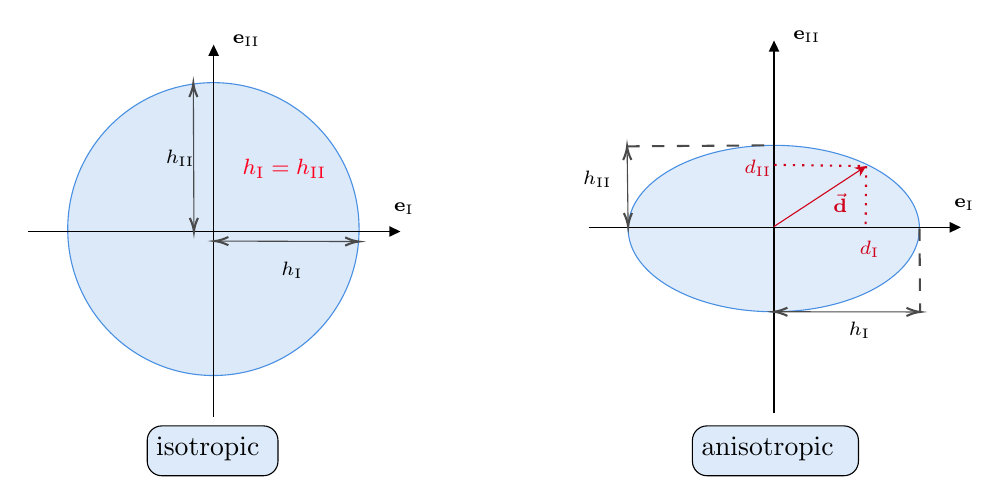
\begin{tikzpicture}[x=0.75pt,y=0.75pt,yscale=-1,xscale=1]
%uncomment if require: \path (0,365); %set diagram left start at 0, and has height of 365

%Shape: Ellipse [id:dp47149657789461774] 
\draw  [color={rgb, 255:red, 74; green, 144; blue, 226 }  ,draw opacity=1 ][fill={rgb, 255:red, 74; green, 144; blue, 226 }  ,fill opacity=0.2 ] (80.03,160.17) .. controls (80.03,121.2) and (111.45,89.62) .. (150.21,89.62) .. controls (188.98,89.62) and (220.4,121.2) .. (220.4,160.17) .. controls (220.4,199.13) and (188.98,230.72) .. (150.21,230.72) .. controls (111.45,230.72) and (80.03,199.13) .. (80.03,160.17) -- cycle ;
%Straight Lines [id:da9023088519674093] 
\draw    (61,161.33) -- (237.33,161.33) ;
\draw [shift={(240.33,161.33)}, rotate = 180] [fill={rgb, 255:red, 0; green, 0; blue, 0 }  ][line width=0.08]  [draw opacity=0] (5.36,-2.57) -- (0,0) -- (5.36,2.57) -- cycle    ;
%Straight Lines [id:da8803342561855532] 
\draw    (150.33,250.67) -- (150.33,74.33) ;
\draw [shift={(150.33,71.33)}, rotate = 90] [fill={rgb, 255:red, 0; green, 0; blue, 0 }  ][line width=0.08]  [draw opacity=0] (5.36,-2.57) -- (0,0) -- (5.36,2.57) -- cycle    ;
%Straight Lines [id:da970968031905884] 
\draw [color={rgb, 255:red, 74; green, 74; blue, 74 }  ,draw opacity=1 ]   (140.83,159.36) -- (140.56,91.95) ;
\draw [shift={(140.55,89.95)}, rotate = 89.77] [color={rgb, 255:red, 74; green, 74; blue, 74 }  ,draw opacity=1 ][line width=0.75]    (6.56,-1.97) .. controls (4.17,-0.84) and (1.99,-0.18) .. (0,0) .. controls (1.99,0.18) and (4.17,0.84) .. (6.56,1.97)   ;
\draw [shift={(140.83,161.36)}, rotate = 269.77] [color={rgb, 255:red, 74; green, 74; blue, 74 }  ,draw opacity=1 ][line width=0.75]    (6.56,-1.97) .. controls (4.17,-0.84) and (1.99,-0.18) .. (0,0) .. controls (1.99,0.18) and (4.17,0.84) .. (6.56,1.97)   ;
%Straight Lines [id:da687532719461613] 
\draw [color={rgb, 255:red, 74; green, 74; blue, 74 }  ,draw opacity=1 ]   (152.86,165.94) -- (218.27,166.17) ;
\draw [shift={(220.27,166.18)}, rotate = 180.2] [color={rgb, 255:red, 74; green, 74; blue, 74 }  ,draw opacity=1 ][line width=0.75]    (6.56,-1.97) .. controls (4.17,-0.84) and (1.99,-0.18) .. (0,0) .. controls (1.99,0.18) and (4.17,0.84) .. (6.56,1.97)   ;
\draw [shift={(150.86,165.94)}, rotate = 0.2] [color={rgb, 255:red, 74; green, 74; blue, 74 }  ,draw opacity=1 ][line width=0.75]    (6.56,-1.97) .. controls (4.17,-0.84) and (1.99,-0.18) .. (0,0) .. controls (1.99,0.18) and (4.17,0.84) .. (6.56,1.97)   ;
%Shape: Ellipse [id:dp2890703530536485] 
\draw  [color={rgb, 255:red, 74; green, 144; blue, 226 }  ,draw opacity=1 ][fill={rgb, 255:red, 74; green, 144; blue, 226 }  ,fill opacity=0.17 ] (350.03,159.91) .. controls (350.03,137.76) and (381.45,119.81) .. (420.21,119.81) .. controls (458.98,119.81) and (490.4,137.76) .. (490.4,159.91) .. controls (490.4,182.05) and (458.98,200) .. (420.21,200) .. controls (381.45,200) and (350.03,182.05) .. (350.03,159.91) -- cycle ;
%Straight Lines [id:da7491324989595073] 
\draw    (331,159.33) -- (507.33,159.33) ;
\draw [shift={(510.33,159.33)}, rotate = 180] [fill={rgb, 255:red, 0; green, 0; blue, 0 }  ][line width=0.08]  [draw opacity=0] (5.36,-2.57) -- (0,0) -- (5.36,2.57) -- cycle    ;
%Straight Lines [id:da5761256453181017] 
\draw    (420.33,248.67) -- (420.33,72.33) ;
\draw [shift={(420.33,69.33)}, rotate = 90] [fill={rgb, 255:red, 0; green, 0; blue, 0 }  ][line width=0.08]  [draw opacity=0] (5.36,-2.57) -- (0,0) -- (5.36,2.57) -- cycle    ;
%Straight Lines [id:da7041621788435982] 
\draw [color={rgb, 255:red, 74; green, 74; blue, 74 }  ,draw opacity=1 ]   (350,157) -- (349.55,122.31) ;
\draw [shift={(349.53,120.31)}, rotate = 89.26] [color={rgb, 255:red, 74; green, 74; blue, 74 }  ,draw opacity=1 ][line width=0.75]    (6.56,-1.97) .. controls (4.17,-0.84) and (1.99,-0.18) .. (0,0) .. controls (1.99,0.18) and (4.17,0.84) .. (6.56,1.97)   ;
\draw [shift={(350.03,159)}, rotate = 269.26] [color={rgb, 255:red, 74; green, 74; blue, 74 }  ,draw opacity=1 ][line width=0.75]    (6.56,-1.97) .. controls (4.17,-0.84) and (1.99,-0.18) .. (0,0) .. controls (1.99,0.18) and (4.17,0.84) .. (6.56,1.97)   ;
%Straight Lines [id:da33821473867960394] 
\draw [color={rgb, 255:red, 74; green, 74; blue, 74 }  ,draw opacity=1 ]   (422.21,200) -- (488.71,200.1) ;
\draw [shift={(490.71,200.1)}, rotate = 180.08] [color={rgb, 255:red, 74; green, 74; blue, 74 }  ,draw opacity=1 ][line width=0.75]    (6.56,-1.97) .. controls (4.17,-0.84) and (1.99,-0.18) .. (0,0) .. controls (1.99,0.18) and (4.17,0.84) .. (6.56,1.97)   ;
\draw [shift={(420.21,200)}, rotate = 0.08] [color={rgb, 255:red, 74; green, 74; blue, 74 }  ,draw opacity=1 ][line width=0.75]    (6.56,-1.97) .. controls (4.17,-0.84) and (1.99,-0.18) .. (0,0) .. controls (1.99,0.18) and (4.17,0.84) .. (6.56,1.97)   ;
%Straight Lines [id:da09564868493828071] 
\draw [color={rgb, 255:red, 208; green, 2; blue, 27 }  ,draw opacity=1 ]   (420.21,159) -- (462.21,131.46) ;
\draw [shift={(464.71,129.81)}, rotate = 146.74] [fill={rgb, 255:red, 208; green, 2; blue, 27 }  ,fill opacity=1 ][line width=0.08]  [draw opacity=0] (5.36,-2.57) -- (0,0) -- (5.36,2.57) -- (3.56,0) -- cycle    ;
%Straight Lines [id:da7191734000127111] 
\draw [color={rgb, 255:red, 74; green, 74; blue, 74 }  ,draw opacity=1 ][line width=0.75]  [dash pattern={on 4.5pt off 4.5pt}]  (349.53,120.31) -- (420.21,119.81) ;
%Straight Lines [id:da23417744915968897] 
\draw [color={rgb, 255:red, 74; green, 74; blue, 74 }  ,draw opacity=1 ][line width=0.75]  [dash pattern={on 4.5pt off 4.5pt}]  (490.4,159.91) -- (490.71,200.1) ;
%Straight Lines [id:da9599209932665848] 
\draw [color={rgb, 255:red, 208; green, 2; blue, 27 }  ,draw opacity=1 ][line width=0.75]  [dash pattern={on 0.84pt off 2.51pt}]  (420.43,129.24) -- (464.71,129.81) ;
%Straight Lines [id:da46869669446608475] 
\draw [color={rgb, 255:red, 208; green, 2; blue, 27 }  ,draw opacity=1 ][line width=0.75]  [dash pattern={on 0.84pt off 2.51pt}]  (464.71,129.81) -- (464.43,160.1) ;

% Text Node
\draw (126,120.73) node [anchor=north west][inner sep=0.75pt]  [font=\scriptsize]  {$h_{\mathrm{II}}$};
% Text Node
\draw (181.67,174.73) node [anchor=north west][inner sep=0.75pt]  [font=\scriptsize]  {$h_{\mathrm{I}}$};
% Text Node
\draw (158.33,65.4) node [anchor=north west][inner sep=0.75pt]  [font=\scriptsize]  {$\mathbf{e}_{\mathrm{II}}$};
% Text Node
\draw (236,146.4) node [anchor=north west][inner sep=0.75pt]  [font=\scriptsize]  {$\mathbf{e}_{\mathrm{I}}$};
% Text Node
\draw (163,125.4) node [anchor=north west][inner sep=0.75pt]  [font=\footnotesize,color={rgb, 255:red, 255; green, 0; blue, 31 }  ,opacity=1 ]  {$h_{\mathrm{I}} =h_{\mathrm{II}}$};
% Text Node
\draw  [fill={rgb, 255:red, 74; green, 144; blue, 226 }  ,fill opacity=0.19 ]  (118.33,262) .. controls (118.33,258.13) and (121.47,255) .. (125.33,255) -- (174.33,255) .. controls (178.2,255) and (181.33,258.13) .. (181.33,262) -- (181.33,272) .. controls (181.33,275.87) and (178.2,279) .. (174.33,279) -- (125.33,279) .. controls (121.47,279) and (118.33,275.87) .. (118.33,272) -- cycle  ;
\draw (121.33,259) node [anchor=north west][inner sep=0.75pt]   [align=left] {isotropic};
% Text Node
\draw (327.05,130.92) node [anchor=north west][inner sep=0.75pt]  [font=\scriptsize]  {$h_{\mathrm{II}}$};
% Text Node
\draw (455.1,203.59) node [anchor=north west][inner sep=0.75pt]  [font=\scriptsize]  {$h_{\mathrm{I}}$};
% Text Node
\draw (428.33,63.4) node [anchor=north west][inner sep=0.75pt]  [font=\scriptsize]  {$\mathbf{e}_{\mathrm{II}}$};
% Text Node
\draw (506,144.4) node [anchor=north west][inner sep=0.75pt]  [font=\scriptsize]  {$\mathbf{e}_{\mathrm{I}}$};
% Text Node
\draw  [fill={rgb, 255:red, 74; green, 144; blue, 226 }  ,fill opacity=0.19 ]  (381,262) .. controls (381,258.13) and (384.13,255) .. (388,255) -- (454,255) .. controls (457.87,255) and (461,258.13) .. (461,262) -- (461,272) .. controls (461,275.87) and (457.87,279) .. (454,279) -- (388,279) .. controls (384.13,279) and (381,275.87) .. (381,272) -- cycle  ;
\draw (384,259) node [anchor=north west][inner sep=0.75pt]   [align=left] {anisotropic};
% Text Node
\draw (460.24,164.78) node [anchor=north west][inner sep=0.75pt]  [font=\scriptsize,color={rgb, 255:red, 208; green, 2; blue, 27 }  ,opacity=1 ]  {$d_{\mathrm{I}}$};
% Text Node
\draw (404.76,125.78) node [anchor=north west][inner sep=0.75pt]  [font=\scriptsize,color={rgb, 255:red, 208; green, 2; blue, 27 }  ,opacity=1 ]  {$d_{\mathrm{II}}$};
% Text Node
\draw (447.71,141.64) node [anchor=north west][inner sep=0.75pt]  [font=\scriptsize,color={rgb, 255:red, 208; green, 2; blue, 27 }  ,opacity=1 ]  {$\vec{\mathbf{d}}$};


\end{tikzpicture}
%
    }
    % \caption{Geometric interpretation of the unit-metric
    % ellipse in physical space}
    \label{fig:metric_ellipse}
\end{figure}

\noindent
We therefore have a geometric description of the
desired anisotropy. The remaining question is how
to construct a metric whose orientation and dimensions
reflect the local variations of the density field.


\subsection{Defining the target size in each direction}

\noindent
This brings us back to the regularized curvature matrix
$\mathbf{K}_\rho$ defined at equation~\ref{eq: regCurv}.
By construction, this matrix already contains the
information required to determine the orientation
and relative dimensions of the metric ellipse.
Nevertheless, $\mathbf{K}_\rho$ alone does not yet
provide a complete physical mesh-size prescription.
We must also be able to specify the absolute scale
of the elements without modifying the directional
information extracted from the density field.
For this purpose, we introduce a positive scaling
factor $\alpha$ and define our local metric as

\begin{equation}
    \boxed{
        \mathbf{M}=\alpha\mathbf{K}_\rho,
        \qquad \alpha>0.
    }
\end{equation}

\noindent
This construction separates two distinct roles:
$\mathbf{K}_\rho$ determines the relative geometry
of the refinement, whereas $\alpha$ controls its
absolute physical scale.
Both matrices share the same
eigenvectors: 

\begin{equation}
    \boxed{
        \lambda_{M,a}=\alpha k_a,
        \qquad a\in\{\mathrm{I},\mathrm{II}\}.
    }
\end{equation}

\noindent
Using the previously established relation between
metric eigenvalues and physical lengths, we obtain

\begin{equation}
    \boxed{
        h_a=\frac{1}{\sqrt{\alpha k_a}},
        \qquad a\in\{\mathrm{I},\mathrm{II}\}.
    }
\end{equation}

\noindent
This expression directly translates the density
curvature into a physical mesh-size prescription:
a large curvature requires a smaller characteristic
length, whereas a weaker curvature allows a larger
spacing between vertices. Moreover, the ratio between the two semi-axes of
the metric ellipse becomes

\begin{equation}
    \boxed{
        \frac{h_{\mathrm{I}}}{h_{\mathrm{II}}}
        =
        \sqrt{
            \frac{k_{\mathrm{II}}}{k_{\mathrm{I}}}
        }.
    }
\end{equation}

\noindent
The orientation and aspect
ratio of the metric ellipse are determined entirely
by $\mathbf{K}_\rho$, while $\alpha$ changes its
overall dimensions without modifying its proportions.
It is therefore important to distinguish between
understanding the role of $\alpha$ and determining
its actual value. The absolute physical dimensions
of the mesh still depend on this factor, which must
eventually be specified.



\subsection{A natural interpretation of the scaling factor}

\noindent
A first way to determine $\alpha$ is to return to
our initial interpolation-error model. We previously established that, for an edge of physical length $h_a$ aligned with an eigenvector $\mathbf{e}_a$
of the density Hessian, the midpoint interpolation
error can be locally approximated by

\begin{equation}
    |E_a|
    \simeq
    \frac{h_a^2}{8}|\lambda_a|.
\end{equation}

\noindent
Substituting the target physical size prescribed
by our metric gives

\begin{equation}
    |E_a|
    \simeq
    \frac{|\lambda_a|}{8\alpha k_a}.
\end{equation}

\noindent
Since the regularized curvature satisfies
$k_a=\max(|\lambda_a|,\varepsilon)$, we obtain
the approximate error bound

\begin{equation}
    \boxed{
        |E_a|\lesssim\frac{1}{8\alpha}.
    }
\end{equation}

\noindent
This relation gives an additional physical
interpretation of $\alpha$: it controls the
characteristic interpolation-error scale
associated with the prescribed metric lengths.
For instance, if we wished to impose a local
interpolation-error tolerance $\epsilon>0$,
a natural choice would be $\alpha=\frac{1}{8\epsilon}$.
Such a choice would be consistent with our
local interpolation-error model and would
determine the target sizes from a prescribed
error tolerance.\\

\noindent
However, in our application, the available
computational resources must also be considered.
Rather than fixing $\alpha$ immediately through
a local error tolerance, we will determine its
distribution later from a global mesh budget.
The scaling factor may therefore vary spatially
to allocate different levels of resolution
across the domain.\\


\noindent   
At this stage, the construction
$\mathbf{M}=\alpha\mathbf{K}_\rho$ is sufficient
to understand how density curvature determines
the local geometry of the adapted mesh.



\subsection{Application to aerodynamic shocks}

\noindent
We can now interpret this construction in the
physical situation that originally motivated
our adaptation method: the resolution of
aerodynamic shocks.
Consider a straight shock, we had :

\begin{equation}
    \mathbf{H}_\rho
    \simeq
    R''(s)\mathbf{n}\mathbf{n}^{\top}
\end{equation}

\noindent
This expression shows that the curvature
is primarily concentrated in the normal
direction.
After applying the previously introduced
regularization, the corresponding principal
curvatures are approximately

\begin{equation}
    k_n=\max\left(|R''(s)|,\varepsilon\right),
    \qquad
    k_t=\varepsilon.
\end{equation}

\noindent
The metric therefore prescribes the following
characteristic physical lengths:

\begin{equation}
    \boxed{
        h_n=\frac{1}{\sqrt{\alpha k_n}},
        \qquad
        h_t=\frac{1}{\sqrt{\alpha k_t}}.
    }
\end{equation}

\noindent
In regions where the normal curvature is
significantly larger than the regularization
threshold, we obtain

\begin{equation}
    k_n\gg k_t
    \qquad\Longrightarrow\qquad
    h_n\ll h_t.
\end{equation}

\noindent
The metric ellipse is therefore strongly
elongated in the tangential direction of
the shock, while its normal semi-axis
remains much shorter.\\

\noindent
This geometry directly reflects the behavior
of the density field. Mesh elements must
have a small characteristic dimension in
the shock-normal direction to better resolve
the rapid density transition, while they may
retain a larger dimension in the tangential
direction, where the density curvature
remains relatively small.


% One limitation must nevertheless be kept
% in mind. At the inflection point of an
% S-shaped numerical shock profile, $R''(s)$
% may vanish even though the density gradient
% remains large.

% A purely Hessian-based indicator may therefore
% locally underestimate the required refinement.
% The regularization ensures that the metric
% remains positive definite, but it does not
% entirely eliminate this limitation of the
% curvature-based indicator.





%%%% to continue%%%%%%%%



\section{Choosing the Node Count and Its Spatial Distribution}

We now know how to determine element shapes and orientations from the density Hessian. But how should we choose their absolute sizes when only a limited number of nodes is available?


% ============================================================
\subsection{Relating Local Element Sizes to the Number of Elements}
% ============================================================

\subsubsection{Why Do Physical Element Sizes Determine the Number of Triangles?}

\noindent
Consider a small region in which the metric varies sufficiently slowly to be regarded as constant. If both $h_{\mathrm I}$ and $h_{\mathrm{II}}$ are halved, the characteristic physical dimensions of the elements are halved in both directions. Their characteristic area is therefore divided by 4 $A_{\mathrm{new}}\simeq\frac{A_{\mathrm{old}}}{4}$.\\

\noindent
Consequently, approximately 4 times as many triangles are required to cover a region with the same physical area. This suggests that the required number of elements per unit physical area is proportional to $\frac{1}{h_{\mathrm I}h_{\mathrm{II}}}$.\\

\noindent
We shall now establish this relationship using the metric tensor.


\subsubsection{How Does the Metric Transform Areas?}
\noindent
We previously used the metric $\|\mathbf d\|_{\mathbf M}^{2}
=\mathbf d^{\top}\mathbf M\mathbf d$ to transform physical lengths. The same principle can be applied to areas.\\ 

\noindent
Since $\mathbf M$ is symmetric positive definite, it has a matrix square root $\mathbf M^{1/2}$. We can therefore define a transformed displacement:

\begin{equation}
\widetilde{\mathbf d}=\mathbf M^{1/2}\mathbf d
\end{equation}
\noindent
By construction,

\begin{equation}
\|\mathbf d\|_{\mathbf M}^{2}
=\widetilde{\mathbf d}^{\top}\widetilde{\mathbf d}
\end{equation}
\noindent
Thus, measuring a length using $\mathbf M$ is equivalent to measuring an ordinary Euclidean length after transforming the displacement through $\mathbf M^{1/2}$. In the eigenvector basis of the metric tensor, the transformation reads

\begin{equation}
\begin{pmatrix}
\widetilde d_{\mathrm I}\\
\widetilde d_{\mathrm{II}}
\end{pmatrix}
=
\begin{pmatrix}
\sqrt{\lambda_{M,\mathrm I}}&0\\
0&\sqrt{\lambda_{M,\mathrm{II}}}
\end{pmatrix}
\begin{pmatrix}
d_{\mathrm I}\\
d_{\mathrm{II}}
\end{pmatrix}.
\end{equation}
\noindent
Lengths are therefore multiplied by $\sqrt{\lambda_{M,\mathrm I}}$ in the first principal direction and by $\sqrt{\lambda_{M,\mathrm{II}}}$ in the second. An area is the product of two independent dimensions. Accordingly, it is scaled by the product

\begin{equation}
\sqrt{\lambda_{M,\mathrm I}}
\sqrt{\lambda_{M,\mathrm{II}}}.
\end{equation}
\noindent
The determinant of a matrix is the product of its eigenvalues $\det\mathbf M
=\lambda_{M,\mathrm I}\lambda_{M,\mathrm{II}}$. Hence, for a locally constant metric,

\begin{equation}
\boxed{
A_M=\sqrt{\det\mathbf M}\,A
}
\end{equation}
\noindent
where $A$ is the physical area and $A_M$ is the corresponding area after the metric transformation. \textbf{The factor $\sqrt{\det\mathbf M}$ measures the dilation of physical area when expressed in metric space.}\\

\noindent
We call then the \emph{metric density}

\begin{equation}
\boxed{
\eta(\mathbf x)=\sqrt{\det\mathbf M(\mathbf x)}
}
\end{equation}


\noindent
The eigenvalues of the metric are related to the target element sizes through $\lambda_{M,a}=\frac{1}{h_a^2}$. It follows that

\begin{align*}
\eta(\mathbf x) =\sqrt{\lambda_{M,\mathrm I}\lambda_{M,\mathrm{II}}}=\sqrt{\frac{1}{h_{\mathrm I}^2h_{\mathrm{II}}^2}}=\frac{1}{h_{\mathrm I}h_{\mathrm{II}}}.
\end{align*}
\noindent
Therefore,

\begin{equation}
\boxed{
\eta(\mathbf x)
=\frac{1}{h_{\mathrm I}h_{\mathrm{II}}}
=\sqrt{\det\mathbf M(\mathbf x)}.
}
\end{equation}
\noindent
It represents \textbf{the local resolution requested by the metric per unit physical area}. However, $\eta$ is not exactly the surfacic number of nodes. It is a geometric quantity proportional to that number when the triangles are close to their target shapes and sizes in metric space.\\
\noindent
\textbf{We now have a local measure of the resolution requirement}. To construct a complete mesh, we must integrate these requirements over the entire domain.

\subsubsection{From Local Density to Global Complexity}
\noindent
First, consider a domain partitioned into small regions $\Omega_q$, each with physical area $A_q$, in which the metric density is approximately constant and equal to $\eta_q$. The metric area associated with region $q$ is $C_q=A_q\eta_q$. \\
\noindent
As the regions become sufficiently small, the sum becomes an integral:

\begin{equation}
\boxed{
C(\mathbf M)
=\iint_\Omega\eta(\mathbf x)\,\mathrm{dA}
=\iint_\Omega\sqrt{\det\mathbf M(\mathbf x)}\,\mathrm{dA}.
}
\end{equation}
\noindent
This quantity is called the \textbf{metric complexity}. It is the continuous sum of the metric areas of the small regions forming the domain. It describes the total amount of geometric resolution requested throughout the domain.\\
\noindent
We must still convert this quantity into a concrete number of triangles and nodes.


\subsubsection{Converting Metric Complexity into a Number of Triangles}

Our method aims to generate triangles whose edges have approximately unit length in metric space. Ideally, these triangles are also nearly equilateral in metric space, even though they may be elongated in physical space.\\

\noindent
Consider an equilateral triangle $T_\triangle$ with side length $1$. Its height is $H_\triangle=\nicefrac{\sqrt{3}}{2}$,and its area is $A_\triangle=\nicefrac{\sqrt{3}}{4}$. If all triangles have approximately this metric area, the total metric complexity is approximately equal to the sum of their metric areas:

\begin{equation}
C(\mathbf M)\simeq N_T\frac{\sqrt{3}}{4},
\end{equation}
\noindent
where $N_T$ is the number of triangles. We therefore obtain

\begin{equation}
\boxed{
N_T\simeq\frac{4}{\sqrt{3}}C(\mathbf M).
}
\end{equation}


\noindent
Since our objective is to control the number of nodes, we must also relate $N_T$ to the total number of vertices $N_V$. For a conformal triangulation of a simply connected planar domain, Euler's relation gives

\begin{equation*}
N_T=2N_V-N_b-2
\end{equation*}
\noindent
where $N_b$ is the number of boundary vertices.\\
\noindent
For a sufficiently large mesh, the boundary contribution is relatively small, and therefore $N_T\simeq 2N_V$.

\noindent
Let $N_\star$ denote the desired number of nodes. Then

\begin{equation}
N_T\simeq 2N_\star
\end{equation}
\noindent
Combining this approximation with the previous relationship gives

\begin{align*}
C_\star=\frac{\sqrt{3}}{4}N_T\simeq\frac{\sqrt{3}}{4}(2N_\star).
\end{align*}
\noindent
Hence,

\begin{equation}
\boxed{
C_\star\simeq\frac{\sqrt{3}}{2}N_\star.
}
\end{equation}
\noindent
\textbf{We have converted our CFD computational constraint---a target number $N_\star$ of nodes---into a mathematical constraint on the metric field:}

\begin{equation}
\iint_\Omega\sqrt{\det\mathbf M(\mathbf x)}\,\mathrm{dA}
\simeq\frac{\sqrt{3}}{2}N_\star
\end{equation}
\noindent
This is the condition we will seek to satisfy when constructing the metric tensor.


\noindent
\textit{The relationship remains approximate in practice: the geometry of the NACA~0012 airfoil, boundary discretization, and elements that do not have exactly unit metric edge lengths all affect the actual node count.}


% ============================================================
\subsection{How Should Nodes Be Distributed to Better Resolve Density?}
% ============================================================

We have obtained a global constraint on the metric:

\begin{equation}
\boxed{
\mathscr{C}=\left\{\eta>0 \mid \iint_\Omega\eta(\mathbf x)\,\mathrm{dA}-C_\star=0\right\}
}
\end{equation}
\noindent
However, this constraint alone does not determine the mesh. Several metric-density distributions can produce the same total complexity. We could generate an almost uniform mesh, concentrate nodes near a shock, or refine other regions of the domain while retaining approximately the same total number of nodes.\\

\noindent
We  need a second criterion to \textbf{select, among all meshes respecting the budget, the one that best represents the density field}. This is precisely the role of our interpolation-error model.\\

\noindent
We previously showed that the linear interpolation error along a principal direction of the density Hessian scales as

\begin{equation*}
|E_a|\simeq\frac18|\lambda_a|h_a^2.
\end{equation*}
\noindent
After regularizing the curvature, the product $k_a h_a^2$ provides a conservative estimate of the error scale, up to a constant factor. In 2D, we have two principal directions. We want to account for the errors associated with both directions simultaneously. A natural choice is to add their contributions:

\begin{equation}
\boxed{
E_\rho
=k_{\mathrm I}h_{\mathrm I}^2
+k_{\mathrm{II}}h_{\mathrm{II}}^2.
}
\end{equation}
\noindent
We call $E_\rho$ our \textbf{local interpolation-error indicator}. To express this indicator directly using matrices, recall that

\begin{equation*}
\mathbf K_\rho
=\mathbf Q
\begin{pmatrix}
k_{\mathrm I}&0\\
0&k_{\mathrm{II}}
\end{pmatrix}
\mathbf Q^\top,\qquad
\mathbf M^{-1}
=\mathbf Q
\begin{pmatrix}
h_{\mathrm I}^2&0\\
0&h_{\mathrm{II}}^2
\end{pmatrix}
\mathbf Q^\top.
\end{equation*}
\noindent
The product $\mathbf M^{-1}\mathbf K_\rho$ therefore has eigenvalues $k_{\mathrm I}h_{\mathrm I}^2$ and $k_{\mathrm{II}}h_{\mathrm{II}}^2$. Since the trace of a matrix equals the sum of its eigenvalues, we can write

\begin{equation}
\boxed{
E_\rho(\mathbf M)
=\operatorname{tr}\!\left(\mathbf M^{-1}\mathbf K_\rho\right).
}
\end{equation}
\noindent
% This matrix expression is useful because it remains valid when the matrices are expressed in another coordinate basis.
\noindent
Since we have already established the optimal form of the metric tensor, we can simplify the error indicator. With $\mathbf M=\alpha\mathbf K_\rho$, we obtain

\begin{equation*}
\mathbf M^{-1}\mathbf K_\rho=\frac{1}{\alpha}\mathbf I.
\end{equation*}
\noindent
Knowing that $\operatorname{tr}\left(\mathbf{I}_{\mathbb{R}^2}\right)=2$, 

\begin{equation}
\boxed{
E_\rho=\frac{2}{\alpha}
}
\end{equation}
\noindent
Furthermore, the determinant of the metric is

\begin{equation*}
\det\mathbf M=\alpha^2\det\mathbf K_\rho.
\end{equation*}
\noindent
The metric density is thus

\begin{equation}
\label{eq:alpha eta}
\boxed{
\eta=\alpha\sqrt{\det\mathbf K_\rho}
}
\end{equation}
\noindent
Solving for $\alpha$ gives

\begin{equation}
\alpha=\frac{\eta}{\sqrt{\det\mathbf K_\rho}}
\end{equation}
\noindent
Substituting this expression into the error indicator yields

\begin{equation}
\boxed{
E_\rho(\mathbf x)
=\frac{2\sqrt{\det\mathbf K_\rho(\mathbf x)}}{\eta(\mathbf x)}
}
\end{equation}
\noindent
This relationship shows that the local error depends on two quantities:

\begin{itemize}
\item $\sqrt{\det\mathbf K_\rho}$ represents the combined intensity of density curvature in the two principal directions.
\item $\eta$ represents the amount of metric resolution allocated locally.
\end{itemize}

\noindent
We can now formulate our node-allocation problem: \textbf{how should $\eta(\mathbf x)$ be chosen throughout the domain to reduce the error while respecting the global budget $C_\star$?}


% ============================================================
\subsection{Determining the Optimal Node Distribution}
% ============================================================

Our objective is now to determine $\eta$ that minimizes the interpolation error while satisfying the metric complexity constraint $\mathcal C$. This constraint is essential to prevent an unbounded increase in the number of mesh nodes, which would be incompatible with our CFD computational budget.\\

\noindent
To achieve this, we need to define a global mathematical measure of the interpolation error over the entire computational domain. Since our domain is 2D, we seek to continuously accumulate the magnitude of the local interpolation error over its surface, which amounts to performing a surface integral.\\

\noindent
A suitable choice is the $p$-th power of the Lebesgue $L^p$ norm, defined over the domain $\Omega$:

\begin{equation}
    \boxed{
    J_p[\eta]
    = \|E_\rho\|_{L^p}^p
    = \iint_\Omega |E_\rho(\mathbf{x})|^p \, \mathrm{d}A,
    \qquad p \geq 1.
    }
\end{equation}
\noindent
Since the mapping $t \mapsto t^p$ is strictly increasing for $t \geq 0$, minimizing $J_p[\eta]$ is equivalent to minimizing the Lebesgue $L^p$ norm itself. The parameter $p$ controls the weight assigned to regions with large errors:

\begin{itemize}
\item $p=1$: minimizes the sum of local errors, weighted by physical areas.
\item $p=2$: penalizes regions with large errors more heavily.
\item Large $p$: increasingly emphasizes the maximum error values.
\end{itemize}
\noindent
Replacing $E_\rho$ by its expression, our optimization problem is written :





\begin{fundamentalproblem}

{\color{OptBlue}\bfseries\small
\textsc{Optimization Problem}
}

\vspace{0.5em}

{\color{OptGrey}\small
For fixed $p\in\mathbb{N}^*$, $C_\star\in \mathbb{R}^+_*$ and
$\mathbf K_\rho:\Omega\to\mathscr S_2^{++}(\mathbb R)$.
}

\vspace{0.6em}

\begin{equation}
\label{eq:main_optimization_problem}
\displaystyle
\min_{\eta\,\in\,\mathscr C(C_\star)}
J_p[\eta]
=
\iint_\Omega
\left(
\frac{2\sqrt{\det\mathbf K_\rho(\mathbf x)}}
{\eta(\mathbf x)}
\right)^p
\mathrm{dA}
\end{equation}

\vspace{-0.4em}

\begin{equation*}
\mathscr C(C_\star)=
\left\{
\eta\in\mathcal{PC}(\Omega;\mathbb R_*^+)
\;\middle|\;
\iint_\Omega\eta(\mathbf x)\,\mathrm{dA} - C_\star =0
\right\}
\end{equation*}

\end{fundamentalproblem}



%%%%% to continue%%%%

\noindent
Now we solve this problem through the Lagrange Multiplier method. For simplicity, let be  $a(\mathbf{x})=2\sqrt{\det{\mathbf{K}_\rho}(\mathbf{x})}$. The problem is re-written : 
\begin{equation}
    \min_{\eta \in \mathscr{C}(C_\star)} \iint_\Omega a(\mathbf{x})^p\,\eta(\mathbf{x})^{-p} \,\mathrm{dA}\;
\end{equation}
\noindent We intorduce only one $\mu\in\mathbb{R}$ multiplier since we have only one integral requirement. The lagrangian function reads :
\begin{equation}
    \mathcal{L}(\eta,\mu)=\iint_\Omega a^p\eta^{-p}\,\mathrm{dA}\;+\; \mu\left(\iint_\Omega\eta\,\mathrm{dA}\,-\,C_\star\right) = \iint_\Omega \left(a^p\eta^{-p}+\mu\eta\right)\,\mathrm{dA}\;+\; \mu C_\star
\end{equation}
\noindent First we go through the stationarity with respect to $\eta$. Since $\eta\in\mathcal{PC}(\Omega;\mathbb R_*^+)$, we do not derivate $\mathcal{L}$ classically. We use the first admissible arbitrary variation of $\eta$ : $\eta_\varepsilon=\eta\,+\,\varepsilon\,\delta\eta$. \\
\noindent At the optimum, we want $\left.
\frac{d}{d\varepsilon}
\mathcal{L}\left(\eta+\varepsilon\,\delta\eta,\mu\right)
\right|_{\varepsilon=0}=0$. Then under the integral of the lagrangian, we have : 
\begin{equation*}
    \iint_\Omega\left(-p\,a^p\eta^{-(p+1)} + \mu\right)\,\delta\eta \, \mathrm{dA} =0
\end{equation*}
\noindent Given the arbitrariness of an admissible $\delta\eta$, we have :
\begin{equation}
    -p\,a^p\eta^{-(p+1)} + \mu = 0 \;\text{on } \Omega
\end{equation}
\noindent Thus,

\begin{equation}
    \label{eq: eta with mu}
    \boxed{
    \eta(\mathbf{x})=\left(\frac{p}{\mu}\right)^{\tfrac{1}{p+1}}\,a(\mathbf{x})^{\tfrac{p}{p+1}}
    }
\end{equation}

\noindent We still need to compute $\mu$ thanks to the constraint of the set  $\mathscr{C}(C_\star)$ :
\begin{align}
    \iint_\Omega\eta(\mathbf{x})\,\mathrm{dA} = C_\star &\xrightarrow[]{\eqref{eq: eta with mu}} \left(\frac{p}{\mu}\right)^{\tfrac{1}{p+1}} \iint_\Omega a(\mathbf{x})^{\tfrac{p}{p+1}} \,\mathrm{dA} = C_\star \nonumber \\[1em]
    \label{eq: mu expression}
    \left(\frac{p}{\mu}\right)^{\tfrac{1}{p+1}} = \dfrac{C_\star}{\displaystyle\iint_\Omega a(\mathbf{x})^{\tfrac{p}{p+1}} \,\mathrm{dA}}  &\xrightarrow[]{\phantom{\eqref{eq: eta with mu}}} \boxed{\mu = p \left(\dfrac{\displaystyle\iint_\Omega a(\mathbf{x})^{\tfrac{p}{p+1}}\, \mathrm{dA}}{C_\star}\right)^{p+1}}
\end{align}

\noindent So we can express $\eta$ :
\begin{equation}
    \label{eq:optimal_metric_density}
    \eta^\star(\mathbf{x})\overset{\eqref{eq: mu expression}}{=}
    \dfrac{
        C_\star\,a(\mathbf{x})^{\frac{p}{p+1}}
    }{
        \displaystyle\iint_\Omega
        a(\mathbf{x})^{\frac{p}{p+1}}
        \,\mathrm{d}A
    }
\end{equation}


\noindent Given the expression of $a$, the optimal metric density reads:

\begin{equation}
    \label{eq:optimal_metric_density_final}
    \boxed{
    \eta_\star=
    \dfrac{
        C_\star
        \left[\det\mathbf K_\rho\right]^{
            \frac{p}{2(p+1)}
        }
    }{
        \displaystyle\iint_\Omega
        \left[\det\mathbf K_\rho\right]^{
            \frac{p}{2(p+1)}
        }
        \,\mathrm{dA}
    }
    }
\end{equation}


\noindent Using the relation \eqref{eq:alpha eta},
the optimal scaling factor $\alpha_\star$ is given by

\begin{equation}
    \label{eq:optimal_alpha}
    \boxed{
    \alpha_\star=
    \dfrac{
        C_\star
        \left[\det\mathbf K_\rho\right]^{
            -\frac{1}{2(p+1)}
        }
    }{
        \displaystyle\iint_\Omega
        \left[\det\mathbf K_\rho\right]^{
            \frac{p}{2(p+1)}
        }
        \,\mathrm{d}A
    }
    }
\end{equation}



\noindent To simplify the expression, we introduce the global
normalization factor $s_\star$, defined as

\begin{equation}
    \label{eq:optimal_global_scaling}
    s_\star =
    \dfrac{
        C_\star
    }{
        \displaystyle\iint_\Omega
        \left[\det\mathbf K_\rho\right]^{
            \frac{p}{2(p+1)}
        }
        \,\mathrm{d}A
    }
\end{equation}

\noindent Consequently, the optimal scaling factor becomes
\begin{equation}
    \alpha_\star =
    s_\star
    \left[\det\mathbf K_\rho\right]^{
        -\frac{1}{2(p+1)}
    }
\end{equation}

\noindent Finally, substituting this result into the relation
$\mathbf M=\alpha\mathbf K_\rho$, we obtain the
\textbf{optimal metric tensor}:

\begin{equation}
    \label{eq:optimal_metric_tensor}
    \boxed{\boxed{
    \displaystyle
    \mathbf M_\star =
    s_\star
    \left[\det\mathbf K_\rho\right]^{
        -\frac{1}{2(p+1)}
    }
    \mathbf K_\rho
    }}
\end{equation}

\medskip

\noindent\textbf{This expression constitutes the central result
of our resolution-budget allocation procedure.}

\medskip

\noindent The optimal metric preserves the previously established
structure $\mathbf M=\alpha\mathbf K_\rho$. However, the
scaling factor $\alpha$ is no longer arbitrary: it is now
explicitly determined by the error minimization criterion
and the prescribed global metric complexity $C_\star$.

\medskip

\noindent The resulting metric combines two contributions:

\begin{itemize}

    \item \textbf{Local adaptation.}
    The factor
    $\left[\det\mathbf K_\rho\right]^{-1/[2(p+1)]}$
    modulates the local metric magnitude according to the
    curvature information contained in $\mathbf K_\rho$.
    This modulation determines how the available resolution
    is distributed throughout the domain.

    \item \textbf{Global normalization.}
    The factor $s_\star$ applies a uniform scaling to the
    entire metric field, ensuring that the prescribed
    complexity constraint is exactly satisfied:
    \begin{equation*}
        \label{eq:optimal_complexity_verification}
        C(\mathbf M^\star)
        =\iint_\Omega\sqrt{\det\mathbf M^\star}
        \,\mathrm{d}A
        =C_\star
    \end{equation*}

\end{itemize}

\noindent Importantly, although the optimal scaling factor
$\alpha_\star$ varies spatially, it multiplies both
eigenvalues of $\mathbf K_\rho$ by the same positive
factor at each point. Therefore, the optimal metric
preserves the local eigenvectors and anisotropy ratios
defined by $\mathbf K_\rho$, while adjusting the local
element sizes to minimize the global error under the
prescribed resolution budget.






% % ============================================================
% \subsection{Computing the Metric on the Existing Mesh}
% % ============================================================

% We have derived an analytical expression for the desired metric tensor:

% \begin{equation}
% \mathbf M(\mathbf x)
% =s_\star
% [\det\mathbf K_\rho(\mathbf x)]^{-1/(2p+2)}
% \mathbf K_\rho(\mathbf x).
% \end{equation}

% In our application, however, we do not have an analytical expression for density throughout the domain. Instead, we know numerical values at the nodes of the current mesh, from which we have reconstructed the Hessian and then the tensor $\mathbf K_\rho$.

% We must therefore adapt the computation of the global coefficient $s_\star$ to this discrete representation.


% \subsubsection{Constructing an Unnormalized Metric}

% We begin by isolating the local part of the metric, which does not yet depend on the global budget:

% \begin{equation}
% \boxed{
% \mathbf M_0(\mathbf x)
% =[\det\mathbf K_\rho(\mathbf x)]^{-1/(2p+2)}
% \mathbf K_\rho(\mathbf x).
% }
% \end{equation}

% We call $\mathbf M_0$ the \emph{unnormalized metric}.

% Since $\mathbf K_\rho$ has already been computed at each vertex $i$, we can directly construct

% \begin{equation}
% \mathbf M_{0,i}
% =[\det\mathbf K_{\rho,i}]^{-1/(2p+2)}
% \mathbf K_{\rho,i}.
% \end{equation}

% The final metric field will be obtained from

% \begin{equation}
% \boxed{
% \mathbf M_i=s_\star\mathbf M_{0,i}.
% }
% \end{equation}

% We only need to compute $s_\star$.


% \subsubsection{Evaluating the Complexity of the Unnormalized Metric}

% By definition, the complexity of $\mathbf M_0$ is

% \begin{equation}
% C_0
% =\int_\Omega\sqrt{\det\mathbf M_0(\mathbf x)}\,\mathrm{dA}.
% \end{equation}

% We can approximate this integral using the triangles of the existing mesh.

% Consider a triangle $T$ with vertices $i,j,\ell$, and let $|T|$ denote its physical area.

% At the three vertices, we have

% \begin{equation}
% \eta_{0,i}=\sqrt{\det\mathbf M_{0,i}},
% \end{equation}

% and similarly for vertices $j$ and $\ell$.

% A simple approximation of the integral over a triangle is the average of the three nodal values:

% \begin{equation}
% \int_T\eta_0(\mathbf x)\,\mathrm{dA}
% \simeq\frac{|T|}{3}
% \left(\eta_{0,i}+\eta_{0,j}+\eta_{0,\ell}\right).
% \end{equation}

% Summing the contributions from all triangles gives

% \begin{equation}
% C_0\simeq
% \sum_{T\in\mathcal T}\frac{|T|}{3}
% \sum_{i\in\mathcal V(T)}\eta_{0,i}.
% \end{equation}

% We can rearrange this sum by vertex rather than by triangle.

% Each vertex $i$ receives one third of the physical area of every incident triangle.

% Define the physical area associated with vertex $i$ by

% \begin{equation}
% \boxed{
% A_i=\frac13\sum_{T\ni i}|T|.
% }
% \end{equation}

% This area is sometimes called the \emph{associated nodal area} or \emph{lumped nodal area}.

% We therefore obtain

% \begin{equation}
% \boxed{
% C_0\simeq\sum_i A_i\sqrt{\det\mathbf M_{0,i}}.
% }
% \end{equation}

% This formula can be used directly in our algorithm: all the required quantities are available on the existing mesh.


% \subsubsection{Determining the Global Normalization Coefficient}

% We now want the final metric to have the target complexity $C_\star$.

% We have

% \begin{equation}
% \mathbf M=s_\star\mathbf M_0.
% \end{equation}

% In 2D, the determinant satisfies

% \begin{equation}
% \det(s_\star\mathbf M_0)=s_\star^2\det\mathbf M_0.
% \end{equation}

% Since $s_\star>0$,

% \begin{equation}
% \sqrt{\det(s_\star\mathbf M_0)}
% =s_\star\sqrt{\det\mathbf M_0}.
% \end{equation}

% Consequently, the complexity of the final metric is

% \begin{align}
% C(\mathbf M)
% &=\int_\Omega\sqrt{\det(s_\star\mathbf M_0)}\,\mathrm{dA}\\
% &=s_\star\int_\Omega\sqrt{\det\mathbf M_0}\,\mathrm{dA}\\
% &=s_\star C_0.
% \end{align}

% We require

% \begin{equation}
% C(\mathbf M)=C_\star.
% \end{equation}

% It is therefore sufficient to choose

% \begin{equation}
% \boxed{
% s_\star=\frac{C_\star}{C_0}.
% }
% \end{equation}

% Using our nodal approximation of $C_0$,

% \begin{equation}
% \boxed{
% s_\star\simeq
% \frac{C_\star}{
% \displaystyle\sum_i A_i\sqrt{\det\mathbf M_{0,i}}
% }.
% }
% \end{equation}

% The final nodal metric tensors are then constructed as

% \begin{equation}
% \boxed{
% \mathbf M_i=s_\star\mathbf M_{0,i}.
% }
% \end{equation}

% This last operation scales all local metrics so that they approximately satisfy the prescribed global complexity.

% We have therefore determined a metric tensor that simultaneously accounts for the local curvature of density, the desired anisotropy, and the available number of nodes.



% ============================================================
\subsection{Computing the Metric on the Existing Mesh}
\label{subsec:discrete_metric}
% ============================================================

\noindent We have established the analytical expression
of the optimal metric tensor in
\eqref{eq:optimal_metric_tensor}. However, the
regularized curvature tensor $\mathbf K_\rho$ is
only known at the vertices of the existing mesh.
We must therefore evaluate the integral appearing
in the normalization factor $s_\star$ numerically.

\medskip

\noindent We use a nodal quadrature over the triangular
mesh $\mathcal T$. For each triangle $T$, the integral
is approximated using the arithmetic mean of the
integrand evaluated at its three vertices:

\begin{equation}
    \begin{aligned}
    \iint_\Omega
    \left[\det\mathbf K_\rho\right]^{
        \frac{p}{2(p+1)}
    }
    \,\mathrm{d}A
    \simeq
    \sum_{T\in\mathcal T}
    \frac{|T|}{3}
    \sum_{i\in\mathcal V(T)}
    \left[\det\mathbf K_{\rho,i}\right]^{
        \frac{p}{2(p+1)}
    }
    \end{aligned}
\end{equation}

\noindent Regrouping the contributions by vertex,
we introduce the \emph{lumped nodal area} $A_i$:

\begin{equation}
    \label{eq:lumped_nodal_area}
    \boxed{
    A_i=\frac{1}{3}
    \sum_{T_{\ni i}}|T|
    }
\end{equation}

\noindent Each vertex thus receives one third of
the physical area of every incident triangle.
Using \eqref{eq:optimal_global_scaling}, the
normalization factor becomes

\begin{equation}
    \label{eq:discrete_global_scaling}
    \boxed{
    s_\star\simeq
    \dfrac{
        C_\star
    }{
        \displaystyle\sum_{i=1}^{N_V}
        A_i
        \left[\det\mathbf K_{\rho,i}\right]^{
            \frac{p}{2(p+1)}
        }
    }
    }
\end{equation}

\noindent Finally, substituting this coefficient into
\eqref{eq:optimal_metric_tensor}, we obtain the
\textbf{optimal metric tensor at each vertex}:

\begin{equation}
    \label{eq:discrete_optimal_metric}
    \boxed{
    \mathbf M_{\star,i}
    =
    s_\star
    \left[\det\mathbf K_{\rho,i}\right]^{
        -\frac{1}{2(p+1)}
    }
    \mathbf K_{\rho,i}
    }
\end{equation}

\noindent By construction, the resulting metric field
satisfies the prescribed complexity under the
adopted nodal quadrature:

\begin{equation}
\label{eq:discrete_complexity}
    \boxed{
    \sum_{i=1}^{N_V}
    A_i\sqrt{\det\mathbf M_{\star,i}}
    =C_\star
    }
\end{equation}

\noindent The continuous optimization problem has
therefore been reduced to a nodal computation,
providing the metric tensors required for the
subsequent anisotropic mesh adaptation.




% ============================================================
\section{Constructing the New Mesh from the Optimal Metric}
\label{sec:metric_remeshing}
% ============================================================

\noindent In the previous sections, we used the density values
on the initial mesh to calculate the optimal nodal metric
$\mathbf M_i^\star$. This metric gives us the information needed
to build a new mesh: its eigenvectors give the main directions,
its eigenvalues give the target element sizes, and the factor
$s_\star$ accounts for the available node budget.

\noindent We now explain how to use these results to generate
an adapted mesh.

% ------------------------------------------------------------
\subsection{Limiting Element Sizes and Aspect Ratios}
% ------------------------------------------------------------

\noindent Our optimization gives the best metric for the chosen
error model and complexity constraint. However, it does not
set limits on the smallest or largest elements. Very small
elements may increase the CFD cost, while very large or highly
stretched elements may create problems for the mesh generator.
We therefore choose three practical limits:
$h_{\min}>0$, $h_{\max}\geq h_{\min}$ and $A_{\max}\geq1$.

\medskip

\noindent We previously showed that $h_a=1/\sqrt{\lambda_{M,a}}$.
At each vertex $i$, the size condition
$h_{\min}\leq h_a\leq h_{\max}$ is therefore equivalent to

\begin{equation}
    \label{eq:metric_eigenvalue_bounds}
    \boxed{
    \frac{1}{h_{\max}^2}
    \leq\lambda_{M,a,i}
    \leq\frac{1}{h_{\min}^2},
    \qquad a\in\{\mathrm I,\mathrm{II}\}.
    }
\end{equation}

\noindent To satisfy these limits, we replace each eigenvalue
of $\mathbf M_i^\star$ by

\begin{equation}
    \label{eq:clipped_metric_eigenvalues}
    \widetilde\lambda_{M,a,i}
    =\min\!\left(\frac{1}{h_{\min}^2},
    \max\!\left(\frac{1}{h_{\max}^2},
    \lambda_{M,a,i}^\star\right)\right).
\end{equation}

\noindent We must also limit the aspect ratio of the metric ellipse.
Let $\widetilde\lambda_{+,i}$ and $\widetilde\lambda_{-,i}$
be the larger and smaller eigenvalues after the size limits.
Using the relation between eigenvalues and physical sizes,
we obtain

\begin{equation}
    \frac{h_{\mathrm{long}}}{h_{\mathrm{short}}}
    =\sqrt{\frac{\widetilde\lambda_{+,i}}
    {\widetilde\lambda_{-,i}}}
    \leq A_{\max}
    \quad\Longleftrightarrow\quad
    \widetilde\lambda_{-,i}
    \geq\frac{\widetilde\lambda_{+,i}}{A_{\max}^2}.
\end{equation}

\noindent If this condition is not satisfied, we increase
only the smaller eigenvalue:

\begin{equation}
    \label{eq:bounded_aspect_ratio}
    \lambda_{+,i}^{\mathrm b}=\widetilde\lambda_{+,i},
    \qquad
    \lambda_{-,i}^{\mathrm b}
    =\max\!\left(\widetilde\lambda_{-,i},
    \frac{\widetilde\lambda_{+,i}}{A_{\max}^2}\right).
\end{equation}

\noindent We call the new tensor $\mathbf M_{\mathrm b,i}$ the
\emph{bounded metric}. Its main directions are unchanged,
but its target sizes and aspect ratio now respect our limits.

% ------------------------------------------------------------
\subsection{Keeping the Target Complexity}
% ------------------------------------------------------------

\noindent Changing the eigenvalues also changes the determinant
of the metric. As a result, the bounded metric may no longer
satisfy the target complexity $C_\star$. We must check the
budget again after applying the limits.

\noindent Let $\mathcal B$ represent the size and aspect-ratio
limits described above. We introduce a positive factor $\beta$
and define

\begin{equation}
    \label{eq:bounded_metric_beta}
    \mathbf M_{\mathrm b,i}(\beta)
    =\mathcal B\!\left(\beta\mathbf M_i^\star\right),
    \qquad\beta>0.
\end{equation}

\noindent Using the nodal areas $A_i$ defined in
\eqref{eq:discrete_complexity}, we calculate the discrete
complexity of this metric:

\begin{equation}
    \label{eq:bounded_metric_complexity}
    C_h(\beta)=\sum_{i=1}^{N_V}
    A_i\sqrt{\det\mathbf M_{\mathrm b,i}(\beta)}.
\end{equation}

\noindent We then adjust $\beta$ until $C_h(\beta)=C_\star$.
We can use the bisection method because $C_h(\beta)$ is
continuous and does not decrease when $\beta$ increases.
This is possible only if the chosen size limits allow the
requested complexity. In particular, we need

\begin{equation}
    \label{eq:feasible_complexity_interval}
    \frac{|\Omega|}{h_{\max}^2}
    \leq C_\star\leq
    \frac{|\Omega|}{h_{\min}^2}.
\end{equation}

\noindent In this way, we keep the global resolution budget
in the discrete calculation. However, the bounded metric
is not necessarily the exact solution of the original
optimization problem. From now on, $\mathbf M_{\mathrm b}$
refers to the bounded and adjusted metric.

% ------------------------------------------------------------
\subsection{Measuring Edges with the Metric}
% ------------------------------------------------------------

\noindent We now need a way to decide whether an edge is too
long or too short. For this, we first define the metric
between the vertices of the initial mesh.

\noindent As for the $P_1$ interpolation of the density,
we use the shape functions $N_i^T$ of each triangle $T$:

\begin{equation}
    \label{eq:interpolated_metric}
    \mathbf M_{\mathrm b}\big|_T
    =\sum_{i\in\mathcal V(T)}
    N_i^T\mathbf M_{\mathrm b,i},
    \qquad N_i^T\geq0,
    \quad\sum_{i\in\mathcal V(T)}N_i^T=1.
\end{equation}

\noindent Because the nodal metrics are positive definite
and the weights are nonnegative, the interpolated metric
is also positive definite. The initial mesh is therefore
used to evaluate the metric at points between its vertices.

\medskip

\noindent Earlier, we defined the metric length of a displacement.
For a small displacement $\mathrm d\mathbf x$, it is

\begin{equation*}
    \mathrm dL_M
    =\sqrt{\mathrm d\mathbf x^\top
    \mathbf M_{\mathrm b}\,\mathrm d\mathbf x}.
\end{equation*}

\noindent Consider an edge joining $\mathbf x_A$ to
$\mathbf x_B$. Let $\mathbf d=\mathbf x_B-\mathbf x_A$.
We describe points along this edge by
$\mathbf x(t)=\mathbf x_A+t\mathbf d$, with $t\in[0,1]$.
Since $\mathrm d\mathbf x=\mathbf d\,\mathrm dt$,
we add the small metric lengths along the whole edge:

\begin{equation}
    \label{eq:edge_metric_length}
    \boxed{
    L_M(A,B)=\int_0^1
    \sqrt{\mathbf d^\top
    \mathbf M_{\mathrm b}(\mathbf x_A+t\mathbf d)
    \mathbf d}\,\mathrm dt.
    }
\end{equation}

\noindent If the metric is almost constant along the edge,
this becomes $L_M\simeq\sqrt{\mathbf d^\top
\mathbf M_{\mathrm b}\mathbf d}$. Otherwise, we evaluate
the integral numerically. In both cases, the edge length
is measured using the \emph{required local resolution},
not only its physical length.

% ------------------------------------------------------------
\subsection{Building the Adapted Mesh}
% ------------------------------------------------------------

\noindent The goal is to obtain a mesh with edges of
approximately unit metric length, $L_M\approx1$, and
triangles that are close to equilateral in metric space.
This is the same geometric assumption used earlier to
relate $C_\star$ to the target number of nodes $N_\star$.

\noindent To guide the mesh changes, we choose two thresholds
$0<\ell_{\mathrm c}<1<\ell_{\mathrm s}$:

\begin{itemize}
    \item \textbf{Split long edges.} If
    $L_M>\ell_{\mathrm s}$, we add a vertex to reduce
    the metric length of the edge.

    \item \textbf{Collapse short edges.} If
    $L_M<\ell_{\mathrm c}$, we can remove an edge,
    provided that the new triangles remain valid and
    the domain boundary is preserved.

    \item \textbf{Improve triangle shapes.} We can
    change the diagonal shared by two triangles or
    move vertices to improve the triangle shapes
    measured in metric space.
\end{itemize}

\noindent We repeat these operations until the edge lengths
and triangle shapes are close enough to their targets.
The \naca{} airfoil and the outer boundary must remain
unchanged. In practice, vertices on these boundaries
must stay on their curves. We also check the final number
of nodes, because $C_\star$ gives only an approximate
prediction of this number.

\medskip

\noindent \textbf{We can now see how the previous results
control the new mesh.} Near a shock, the density changes
mainly in the normal direction, so we generally have
$k_n\gg k_t$. Before applying the practical limits,
the optimal metric is proportional to $\mathbf K_\rho$.
The target sizes therefore satisfy

\begin{equation}
    \label{eq:shock_target_aspect_ratio}
    \boxed{
    \frac{h_n}{h_t}
    =\sqrt{\frac{k_t}{k_n}}\ll1.
    }
\end{equation}

\noindent This result has a direct meaning for the mesh:
we need short edges across the shock, while longer edges
can be used along the shock. The aspect-ratio limit may
reduce this difference, but it keeps the same directions.
In regions with lower curvature, larger elements are
possible. The global factor calculated earlier controls
how this resolution is shared across the domain.


\begin{figure}[htbp]
\centering
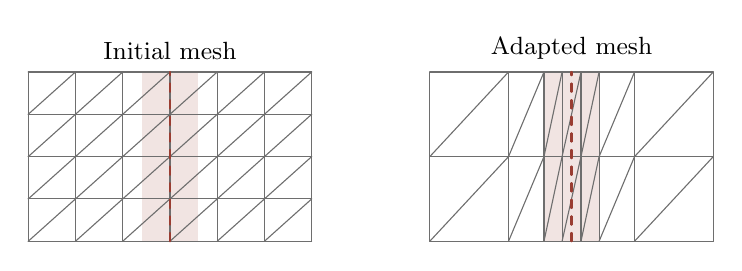
\begin{tikzpicture}[font=\small,line cap=round]
  \begin{scope}
    \fill[shockred!14] (1.45,0) rectangle (2.15,2.15);
    \foreach \x in {0,.6,1.2,1.8,2.4,3,3.6}
      \draw[black!57] (\x,0) -- (\x,2.15);
    \foreach \y in {0,.5375,1.075,1.6125,2.15}
      \draw[black!57] (0,\y) -- (3.6,\y);
    \foreach \x in {0,.6,1.2,1.8,2.4,3}
      \foreach \y in {0,.5375,1.075,1.6125}
        \draw[black!57] (\x,\y) -- ++(.6,.5375);
    \draw[shockred,thick,dashed] (1.8,0) -- (1.8,2.15);
    \node[above] at (1.8,2.19) {Initial mesh};
  \end{scope}
  \begin{scope}[xshift=5.1cm]
    \fill[shockred!14] (1.45,0) rectangle (2.15,2.15);
    \foreach \x in {0,1.0,1.45,1.68,1.92,2.15,2.6,3.6}
      \draw[black!57] (\x,0) -- (\x,2.15);
    \foreach \y in {0,1.075,2.15}
      \draw[black!57] (0,\y) -- (3.6,\y);
    \foreach \xa/\xb in {0/1.0,1.0/1.45,1.45/1.68,1.68/1.92,1.92/2.15,2.15/2.6,2.6/3.6} {
      \draw[black!57] (\xa,0) -- (\xb,1.075);
      \draw[black!57] (\xa,1.075) -- (\xb,2.15);
    }
    \draw[shockred,thick,dashed] (1.8,0) -- (1.8,2.15);
    \node[above] at (1.8,2.19) {Adapted mesh};
  \end{scope}
\end{tikzpicture}

\label{fig:remaillage}
\end{figure}
\FloatBarrier

\noindent We have now connected the density Hessian to the
new mesh geometry. The tensor $\mathbf K_\rho$ gives the
directions and relative sizes, the optimization gives the
local distribution of resolution, and $C_\star$ controls
the overall budget. We can then solve the CFD problem on
the adapted mesh and repeat the process if needed.




























% ============================================================
\section{Iterative Mesh Adaptation and Convergence}
\label{sec:iterative_adaptation}
% ============================================================

\noindent The previous sections have shown how to build a new
mesh from the density field. However, the density itself
comes from a CFD calculation and depends on the mesh used.
The adapted mesh must therefore be tested with a new flow
calculation. This is the last step of our method.

\subsection{Recomputing the Flow}

\noindent Let $\mathcal T^{(k)}$ be the mesh at iteration $k$,
and let $\rho^{(k)}$ be the density obtained after solving
the CFD problem on this mesh. We use this density to
reconstruct the Hessian, calculate the optimal metric,
apply the practical bounds, and generate a new mesh
$\mathcal T^{(k+1)}$.

\noindent We then solve the flow again on $\mathcal T^{(k+1)}$,
using the same flight conditions and boundary conditions.
This gives a new density field $\rho^{(k+1)}$. The full
adaptation cycle can be written as

\begin{equation}
    \label{eq:mesh_adaptation_cycle}
    \begin{aligned}
    \rho^{(k)}
    &\longrightarrow\widehat{\mathbf H}^{(k)}_\rho
    \longrightarrow\mathbf K_\rho^{(k)}
    \longrightarrow\mathbf M_\star^{(k)}\\
    &\longrightarrow\mathbf M_{\mathrm b}^{(k)}
    \longrightarrow\mathcal T^{(k+1)}
    \longrightarrow\rho^{(k+1)}.
    \end{aligned}
\end{equation}

\noindent This new density field may show a sharper shock
or a slightly different shock position. If needed, we
repeat the cycle so that the next metric is based on the
updated solution rather than on the initial mesh.

\subsection{Checking Convergence}

\noindent A finer mesh does not automatically give a more
accurate solution. We must check whether the calculated
flow becomes stable as the mesh is adapted. For this, we
compare density profiles along fixed lines crossing the
shock. Because the meshes have different nodes, the
profiles must be evaluated at the same physical points
$\mathbf x_j$, with $j=1,\ldots,N_s$.

\noindent We can measure the change between two successive
profiles with the relative indicator

\begin{equation}
    \label{eq:density_iteration_change}
    \boxed{
    \delta_\rho^{(k)}=
    \sqrt{
    \dfrac{
        \displaystyle\sum_{j=1}^{N_s}
        \left[\rho^{(k+1)}(\mathbf x_j)
        -\rho^{(k)}(\mathbf x_j)\right]^2
    }{
        \displaystyle\sum_{j=1}^{N_s}
        \left[\rho^{(k)}(\mathbf x_j)\right]^2
    }}.
    }
\end{equation}

\noindent A small value of $\delta_\rho^{(k)}$ means that
the sampled density profiles change little between the
two iterations. We also check the shock position, the
densities on both sides of the shock, and the width of
the numerical transition. These checks help us detect
changes that a single global indicator could miss.

\noindent Finally, we check the mesh itself: its number
of vertices $N_V$, its metric edge lengths, and the
quality of the triangles. In particular, the actual
number of vertices should remain close to the target
$N_\star$, while respecting the geometry of the \naca{}
airfoil and the outer boundary.

\noindent We can stop the adaptation when the CFD solution
is converged on each mesh, the density profiles and shock
position change by less than chosen tolerances, and the
mesh satisfies the required size and quality conditions.
These checks provide evidence of numerical stabilization;
they do not, on their own, prove that the exact flow
solution has been reached.

\subsection{Overall Result of the Method}

\noindent We can now connect all the steps of our work.
The Hessian identifies where the density has strong
curvature and in which directions it changes. The tensor
$\mathbf K_\rho$ turns this information into target
shapes. The optimization determines how to distribute
the available resolution under the budget $C_\star$.
The mesh generator uses the resulting metric to change
the sizes and directions of the triangles. A new CFD
calculation then shows how these changes affect the
computed density.

\medskip

\noindent\textbf{The aim is not simply to produce a finer
mesh, but to place the available nodes where our error
model predicts that they are most useful.} Repeating the
process allows the mesh to follow the flow solution as
it changes, while keeping the computational cost under
control.


\end{document}
